\documentclass[12pt, rectanglelogo]{ociamthesis}

%input macros (i.e. write your own macros file called mymacros.tex 
%and uncomment the next line)
%\include{mymacros}
\usepackage{numprint}
\usepackage[hidelinks]{hyperref}
\usepackage{layouts}

\title{Symmetric instability in the
        Atlantic Meridional Overturning Circulation}   %note \\[1ex] is a line break in the title

\author{Fraser William Goldsworth}
\college{St Anne's College}
\degree{Doctor of Philosophy}
\degreedate{Trinity 2022}

%end the preamble and start the document
\begin{document}

%set the number of sectioning levels that get number and appear in the contents

\maketitle

\begin{romanpages}

\pagestyle{fancy}
\fancypagestyle{plain}{%
  \renewcommand{\headrulewidth}{0pt}
  \fancyhf{}
  \fancyfoot[C]{\usefont{T1}{PTSans-TLF}{m}{n}{\thepage}}
}
\renewcommand{\headrulewidth}{0pt}
\fancyhf{}
\fancyfoot[C]{\usefont{T1}{PTSans-TLF}{m}{n}{\thepage}}

%\cleardoublepage
\phantomsection
\addcontentsline{toc}{chapter}{Dedication}
\begin{dedication}
    For potential vorticity enthusiasts everywhere.
\end{dedication}

\cleardoublepage
\phantomsection
\addcontentsline{toc}{chapter}{Acknowledgements}
\begin{acknowledgements}
    \begin{spacing}{1.25}
    First off I'd like to thank my wonderful supervisors, David and Helen, for all their guidance and support on my DPhil journey. No matter how busy they've been, they've always found time for me. I couldn't have asked for a better team than them.

    I'd also like to thank Elizabeth Yankovsky and three anonymous reviewers for their invaluable feedback on the contents of chapters two, three \& four.
    
    For introducing me to the world of OSNAP and her help with chapter five, I'd like to say a huge thanks to Isabela Le Bras.
    
    For taking me to sea and successfully getting me back home when the plague took hold, thanks to the RAPID AMOC team and the crew on board JC192.
    
    Starting out, I hadn't realised the definition of symmetric instability was so contentious, so thanks to Brian Hoskins and James Maddison for reassuring me it really is as simple as $fQ < 0$.
    
    Behind the scenes, I've been supported by some wonderful friends, so in no particular order, I'd like to say a huge thank you to Beth, Nick, Stuart and anyone else I've spent too much time in the AOPP kitchen with, the Oxford Ocean Climate group, Nilani, the Breakfast Club, Simon and the Oxford University Yacht Club, the 2018 cohort of the NERC DTP, and Lilly.
    
    Finally, a heartfelt thanks to my family who've been my biggest supporters throughout.

    I am grateful for the financial support of the Natural Environment Research Council (NE/L002612/1). Also, this work used the ARCHER2 UK National Supercomputing Service (\url{https://www.archer2.ac.uk}).
    \end{spacing}
\end{acknowledgements}
\begin{abstract}
\usefont{T1}{PTSerif-TLF}{m}{n}
Something abstract.

an ew
\end{abstract}
\tableofcontents

\newpage
\listoffigures
\addcontentsline{toc}{chapter}{List of figures}
\end{romanpages}

%now include the files of latex for each of the chapters etc

\renewcommand{\chaptermark}[1]{%
  \markboth{\usefont{T1}{PTSans-TLF}{m}{n}{#1}}{}
}

\pagestyle{fancy}
\fancyhead[LE, RO]{\usefont{T1}{PTSans-TLF}{m}{n}{\thepage}}
\fancyhead[RE]{\usefont{T1}{PTSans-TLF}{m}{n}{\chaptername\ \thechapter}}
%\fancyhead[LO]{\chaptermark}
\fancyfoot{}

\fancypagestyle{plain}{%
  \renewcommand{\headrulewidth}{0pt}
  \fancyhf{}
  \fancyfoot[C]{\usefont{T1}{PTSans-TLF}{m}{n}{\thepage}}
}

\chapter{Introduction}
\begin{quote}
\textit{The shape of the sea is always the same. Or rather it's always different, but in the same way.} --- Philip Marsden
\end{quote}

\section{The Atlantic Meridional Overturning Circulation}
\begin{itemize}
    \item Introduce the AMOC
    \item Explain how and why it's important
    \item Talk about how our understanding has changed in recent times
    \item Not a conveyor but variability and mesoscale features
    \item Introduce the idea that sub-mesoscale instabilities may play a role
    \item Talk about water mass formation, transformation, and diapycnal mixing
    \item Talk about the processes missing from the water mass budget.
\end{itemize}

\subsection{The Western Boundary Current Systems of  the Tropical Atlantic}

\subsection{The Irminger Current}

\section{Potential vorticity \& symmetric instability}
\begin{itemize}
    \item Describe the character of symmetric instability
    \item Introduce PV and the instability criteria
    \item Touch on links to inertial and gravitational instability but direct the reader to chapter 2 for more depth
    \item Lead into the subsections which describe ways of making potential vorticity negative.
\end{itemize}

Symmetric instability is a type of submesoscale instability that generates overturning cells in a plane perpendicular to a mean flow. The overturning cells tend to be oriented so that they are parallel to isopycnal surfaces, and so symmetric instability is often said to produce slantwise convection. Although the instability leads to mixing predominantly along isopycnals, it can also induce diapycnal mixing. Secondary shear instabilities further enhance this mixing.

Symmetric instability is intimately linked to the scaler quantity, Ertel potential vorticity. In the ocean this is defined as
\begin{equation}
    \label{eq:PVDefinition}
    Q = (\mathbf{f} + \curl{\mathbf{u}})\cdot\grad b    
\end{equation}
where $\mathbf{f}$ is the planetary vorticity vector, $\mathbf{u}$ is the velocity field in the rotating frame of reference, and $b = -  g \flatfrac{\rho}{\rho_0}$ is the buoyancy field. $g$ is gravitational acceleration and $\rho_0$ is a constant reference density. One can interpret the potential vorticity as either the component of absolute vorticity normal to isopycnal surfaces and scaled by the isopycnal thickness, or the stratification along a vortex tube and scaled by the absolute vorticity of the vortex, with the former being the most common way of understanding the quantity.

In a fluid subjected to no momentum or buoyancy forcing, potential vorticity is materially conserved, i.e.
\begin{equation}
    \frac{DQ}{Dt} = 0 \, .
\end{equation}
This means if we follow an individual fluid parcel around we expect its potential vorticity to remain constant. This is a fundamental material invariant which arises from a particle relabelling symmetry on isopycnal surfaces in an inviscid fluid~\citep{Salmon1998}.

If a fluid is subject to external or dissipative momentum and buoyancy forcings the conservation of potential vorticity  becomes
\begin{equation}
    \frac{DQ}{Dt} = \dot{\mathbf{\zeta}} \cdot  \grad{b} + \mathbf{\zeta} \cdot \grad{\dot{b}}
\end{equation}
where $\mathbf{\zeta}$ is the absolute vorticity of the field and a $\,\cdot{}\,$ above a quantity represents its material derivative.

A necessary but not sufficient condition for the excitement of symmetric instability is that the vertical component of planetary vorticity and the potential vorticity of a fluid have opposite signs. Mathematically we require that
\begin{equation}
    \label{eq:PVConservation}
    f Q < 0 \, ,
\end{equation}
where $f$ is the vertical component of the planetary vorticity vector, also known as the Coriolis parameter. Waters which satisfy this instability criterion are often described as having anomalous potential vorticity.

The overturning cells generated during the excitement of symmetric instability causes the mixing of waters with anomalous potential vorticity. The momentum and stratification of the fluid are reconfigured by this mixing, producing waters with potential  vorticity of approximately zero. This corresponds to the absolute vorticity vector being parallel to isopycnal surfaces.

Consider now a fluid initially stable to symmetric instability. For it to become symmetrically unstable we must make the quantity $fQ$ negative. There are then two distinct ways to generate symmetric instability in such a fluid: the first is to change the sign of the planetary vorticity, and the second is to change the sign of the potential vorticity.

\subsection{Ekman driven symmetric instability}
\begin{itemize}
    \item can diffusion generate symmetric instability?
\end{itemize}

\subsection{Cross equatorial symmetric instability}
At the equator planetary vorticity changes from being positive in the northern hemisphere to negative in the southern hemisphere. If we consider a fluid parcel originating in one hemisphere, its potential vorticity will typically match the planetary vorticity so as to ensure symmetric stability. We can than imagine advecting this fluid parcel across the equator. As potential vorticity is materially conserved and planetary vorticity changes sign at the equator, we would expect the symmetric instability criterion to be satisfied in the new hemisphere.

This mechanism does not involve buoyancy or momentum forcing, processes which typically must occur in either a surface or bottom boundary layer. This means symmetric instability resulting from a change in sign of planetary vorticity may occur in the ocean interior and has a distinct character when compared to boundary layer instability. A number of recent observational and theoretical studies have investigated the excitement of symmetric instability resulting from the cross-equatorial change in sign of planetary vorticity, notably CITATIONS. These studies have, however, focused on weak circulations in the ocean interior as opposed to vigorous western boundary currents. In these western boundary currents there is a constant supply of waters with large magnitude, anomalous potential vorticity. These equatorial western boundary currents are rich with temporally varying features, such as mesoscale eddies which interact differently with symmetric instabilities depending on the flow regime.

\begin{figure}
    \centering
    
\includegraphics[width=0.5\textwidth]{oxlogo.eps}
    \caption{Caption}
    \label{fig:my_label}
\end{figure}
\chapter{Symmetric instability}
\begin{quote}
    \textit{In real life there is no algebra} --- Audrey Horne
\end{quote}

In this chapter we will explore the theory behind symmetric instability and its sub-classificaitons. We will start by considering the classical problem of the stability of an inviscid, symmetric, parallel shear flow and then build on this framework to explore different linear stability problems, and how they apply to real-world currents.

\section{Inviscid symmetric instability of parallel shear flow}
\label{sec:InviscidInstabilities}
    In this section we will derive some of the classical results concerning the properties of symmetric instability, by considering the stability of an inviscid parallel shear flow on an $f$-plane. In subsequent sections we will build on this classical analysis to investigate how these properties change in less idelised scenarios.

    The Boussinesq equations of motion for a meridionally symmetric, inviscid flow on an $f$-plane are
    \begin{subequations}
    \label{eqs:InviscidBoussinesq}
    \begin{equation}
        % \bigg( \pdv{t} + u \pdv{x} + w \pdv{z} \bigg)
        \frac{Du}{Dt} - fv - \pdv{\phi}{x} = 0 \, ,
    \end{equation}
    \begin{equation}
        \frac{Dv}{Dt} + fu = 0 \, ,
    \end{equation}
    \begin{equation}
        \frac{Dw}{Dt} - \pdv{\phi}{z} - b = 0 \, ,
    \end{equation}
    \begin{equation}
        \pdv{u}{x} + \pdv{w}{z} = 0 \, ,
    \end{equation}
    and
    \begin{equation}
        \frac{Db}{Dt} = 0 \, .
    \end{equation}
    \end{subequations}
Here, $u$, $v$ \& $w$ are the zonal, meridional \& vertical components of velocity, $f$ is the Coriolis parameter, $\phi$ is the geopotential pressure and $b$ is the buoyancy.

    We now consider a flow which is, initially, purely meridional, with $(u, v, w) = (0, V, 0)$, $\phi = \Phi$ and $b = B$. The flow is steady and both geostrophic and hydrostatic balance. Mathematically
    \begin{subequations}
    \label{eqs:InviscidAssumptions}
    \begin{equation}
        f V = \pdv{\Phi}{x} \, ,
    \end{equation}
    \begin{equation}
        B = \pdv{\Phi}{z} \, ,
    \end{equation}
    \begin{equation}
        \pdv{B}{z} = N^2 \, ,
    \end{equation}
    and
    \begin{equation}
        \pdv{B}{x} = M^2 \, .
    \end{equation}
    \end{subequations}
    We can then perturb this balanced flow, giving perturbed variables $(u, v, w) = (u', V + v', w')$, $\phi = \Phi + \phi'$ and $b = B + b'$. Substituting these values into the equations of motion and considering terms only of linear order or lower in the perturbed variables, we find that
    \begin{subequations}
    \label{eqs:InviscidPerturbed}
    \begin{equation}
        \label{eq:ZonalMomentum}
        % geostrophic balance
        \pdv{u'}{t} - fv' + \pdv{\phi '}{x} = 0 \, ,
    \end{equation}
    \begin{equation}
        \pdv{v'}{t} + u' \pdv{V}{x} + w' \pdv{V}{z} + fu' = 0 \, ,
    \end{equation}
    \begin{equation}
        \label{eq:VerticalMomentum}
        % Hydrostatic balance
        \pdv{w'}{t} + \pdv{\phi '}{z} - b' = 0 \, ,
    \end{equation}
    \begin{equation}
        \pdv{b'}{t} + w' \pdv{B}{z} + u' \pdv{B}{x} = 0 \, ,
    \end{equation}
    and
    \begin{equation}
        \label{eq:Continuity}
        \pdv{u'}{x} + \pdv{w'}{z} = 0 \, ,
    \end{equation}
    \end{subequations}

    From equation~(\ref{eq:Continuity}) we see that we can write $u'$ and $w'$ in terms of an overturning streamfunction $\psi$, where $u' = - \partial_z \psi$ and $w' = \partial_x \psi$. We will now aim to obtain an equation of motion for the overturning streamfunction. The first step is to differentiate the horizontal and vertical momentum equations (equations~\ref{eq:ZonalMomentum} and~\ref{eq:VerticalMomentum}) with respect to the vertical and zonal coordinates respectively. Subtracting the two equations, differentiating with respect to time, and substituting in our equations for $\partial_t b'$ and $\partial_t v'$ gives
    \begin{equation}
    \label{eq:OriginalHoskins}
    \pdv[2]{}{t} \bigg(\pdv[2]{}{x} + \pdv[2]{}{z}\bigg) \psi + \bigg( N^2 \pdv[2]{}{x} - 2 f \pdv{V}{z} \pdv[2]{}{x}{z} + f \zeta \pdv[2]{}{z} \bigg) \psi = 0 \, .
    \end{equation}
    This equation is the Hoskins-Ooyama equation \citep{Hoskins1974, Ooyama1966} and it describes how overturning motions develop within a parallel shear flow, and their dependence on the background flow and its stratification.
    
    \subsection{The instability criterion}
    \label{subsec:InstabilityCriterion}
    To examine the stability of solutions to equation~\ref{eq:OriginalHoskins}, \citet{Hoskins1974} proposes a trial soltuion of the form $\psi = e^{i k(x\sin\phi + z\cos \phi) + i \omega t}$, where $\omega$ is the oscillatory frequency of the perturbations, $k$ the wavenumber, and $\phi$ the angle the perturbation makes with the horizontal. Substituting this into equation~\ref{eq:OriginalHoskins} we find that
    \begin{equation}
        \label{eq:GrowthRate}
        \omega^2 = \cos^2\phi (N^2 \tau^2 - 2f\partial_zV\tau + f\zeta) \, ,
    \end{equation}
    where $\tau = \tan\phi$. If $\omega^2$ is less than zero then the corresponding overturning mode will grow exponentially. For this to occur, the discriminant of the quadratic expression in the above must be negative, i.e. we need $N^2 f \zeta - (f\partial_z V)^2 < 0$. Note that not \textit{all} modes will be unstable if this is the case as the growth rate still depends on the orientation of the perturbations, $\phi$. It is true, however, that if $N^2 f \zeta - (f\partial_z V)^2 \geq 0$ all of the overturning modes will be stable. The instability criteria can be simplified somewhat by noting that as the flow under consideration is in geostrophic balance, $f\partial_zV$ = $\partial_x B$, and so we can wewrite the instability criteria as
    \begin{equation}
        f \bigg[\bigg(f + \pdv{V}{x}\bigg)\pdv{B}{z} - \pdv{V}{z}\pdv{B}{x}\bigg] < 0 \, .
    \end{equation}
    The term in square brackets is recognisable as the potential vorticity of the background flow and so the classical instability criterion of
    \begin{equation}
        f Q < 0
    \end{equation}
    is recovered.

    \subsection{Orientation of the least stable modes}
    From equation~\ref{eq:GrowthRate} we can see that $\omega$ depends on the direction of the perturbation, and so there should be some value of $\phi$ which maximises the growth rate --- i.e. minimses $\omega^2$. The maxima and minima of $\omega^2$ can be found by differentiating eqaution~\ref{eq:GrowthRate} with respect to $\phi$ and setting the result to zero. The extrema of $\omega^2$ then satisfy
    \begin{equation}
        \sin(2 \phi + \arctan(-\frac{2M^2}{N^2 - f \zeta})) = 0 \, .
    \end{equation}
    We can simplify this somewhat if we assume that $\abs{N^2} \gg \abs{f \zeta}$ and that $\abs{N^2} \gg \abs{M^2}$, to give
    \begin{equation}
        \label{eq:UnstableDirections}
        \sin\big(2(\phi - \phi_{iso})\big) = 0 \, ,
    \end{equation}
    where $\phi_{iso}$ is the angle the isopycnals make to the horizontal. This equation has four solutions, corresponding to $\phi$ being either parallel or perpendicular to $\phi_{iso}$. By evaluating the second order derivative of equation~\ref{eq:GrowthRate} we can determine the character of the extrema. We find that with stable stratification, the modes parallel to the isopycnals give minima of $\omega^2$ whereas the modes perpendicular give maxima. Note that the sign of the maxima and minima may be either positive or negative depending on the parameters of the flow, so these modes may be either entirely stable, entirely unstable or a mix of the two.

    In the presence of instability, assuming the isopycnal slope isn't ``too'' steep, and the stratification is stable, the fastest growing mode will be that which is parallel to isopycnals. The growth rate is independent of the magnitude of the wavenumber, however, in the ocean we typically have $\abs{k \sin\phi_{iso}} \ll \abs{k \cos\phi_{iso}}$ and so the the fastest growing modes will tend to have a larger horizontal length scale than in the vertical.

    \subsection{Gravitational \& inertial instability as limiting cases of symmetric instability}
    \citet{Xu1985} explore in detail, how under appropriate coordinate transformations the equations describing the evolution of symmetric instability are mathematically similar to those describing either inertial instability or gravitational instability (an idea first proposed in~\citet{Hoskins1974}). This leads to a useful corallory, that symmetric instability is in many ways a hybrid of gravitational and inertial instability~\citep[e.g.][]{Haine1998}. To understand this we can perform a simple thought experiment.

    Consider a flow, which is free of vertical shear, and therefore has horizontal isopycnals. In this scenario, we have maxima and minima in $\omega^2$ for perturbations which are either purely horizontal or purely vertical. Evaluating $\omega^2$ we find that the two vertical modes correspond to oscillations (or exponentially growing modes if the stratification is unstable) at the Brunt-V\"ais\"al\"a frequency --- this corresponds to gravitational instability. The two horizontal modes correspond to either inertial oscillations or the excitement of inertial instability (depending on the sign of $f \zeta$).

    In the limit of weakly sloping isopycnals, symmetric instability becomes equivalent to inertial instability occuring along isopycnals. Another (and slightly less intuitive) interpretation is that it is equivalent to gravitational instability along isolines of absolute vorticity. Both these interpretations can be traced back the interpretation of potential vorticity as either the absolute vorticity normal to an isopycnal surface or the stratification along absolutely vorticity isolines.
    
    \subsection{Energetics of the instability}
    The rate of change of the kinetic energy of the perturbations is given by
    \begin{equation}
        \label{eq:TurbulentKE}
        \pdv{E_k}{t} = \frac{1}{2}\frac{\partial}{\partial t} (u'^2 + v'^2 + w'^2) \, .
    \end{equation}
    Substituting in equations~\ref{eq:ZonalMomentum} to~\ref{eq:VerticalMomentum}, we can show that this gives
    \begin{equation}
        \pdv{E_k}{t} = - v' (\mathbf{u}'\cdot \grad) V - (\mathbf{u}'\cdot \grad) \phi ' + w' b' 
    \end{equation}
    The first term on the right hand side gives the shear production. It corresponds to a transfer of energy from the shear of the mean flow to the turbulent. The term is occasionally split into a ``geostrophic'' and ``lateral'' shear production term. Typically the excitement of symmetric instability leads to to the excitement of overturning cells oriented along isopycnals, with a horizontal length scale much greater than the vertical. If the turbulent motion is along isopycnals then this term can be thought of as an extraction of energy from the along isopycnal shear of the mean flow.
    
    The second term on the right hand side is the turbulent pressure work term. Using incompressibility of the turbulent flow we can show that
    \begin{equation}
       - (\mathbf{u}'\cdot \grad) \phi ' = - \div{(\mathbf{u'}\phi ')} \, .
    \end{equation}
    This leads to the interpretation of the pressure work term as being a flux. Due to the no normal flow boundary condition, we know this flux must be zero at the boundaries, and all this term does is advect turbulent kinetic energy around the domain, rather than increase the total turbulent kinetic energy. As such it's relatively boring and we won't consider it any further.
    
    The final term in equation~\ref{eq:TurbulentKE} is the turbulent buoyancy flux and corresponds to the turbulent flow extracting gravitational potential energy from the advection of buoyancy anomalies.

    \subsection{The classical and energetic definitions of symmetric instability}
    In the above (and in what follows), we have been referring to the overturning instability that occurs when the potential vorticity of a flow has the opposite sign to the planetary vorticity. We refer to this as the \textit{classical} definition of symmetric instability, as proposed by~\citet{Hoskins1974}. Under this definition, gravitational and inertial instability are both special cases of symmetric instability. 
    
    This isn't, however, the only definition of symmetric instability. \citet{Thomas2013} propose a fine-grained taxonomic system, in which diiferent instabilities can be distinguished by their energy source and the source of their anomalous potential vorticity. They define symmetric instability as getting its energy from the geostrophic shear of the mean flow, inertial instability as getting its energy from the lateral shear of the mean flow and gravitatational instability as getting its energy from buoyancy fluxes. Under these definitions we can have any of pure inertial, hybrid inertial symmetric, pure symmetric, hybrid symmetric gravitational, and pure gravitational instabilities. We refer to this as the \textit{energetic} defintion of symmetric instabilities.

    For the purposes of this work we adopt the classical definition. This is a purely aesthetic choice --- we enjoy the simplicity of the definition and how it preserves the link between symmetric instability, pure gravitational and pure inertial instabilities, potential vorticity, and the extraction of turbulent kinetic energy from along isopycnal shear.

\section{Inviscid symmetric instability of axisymmetric flow}
Parallel shear flow in geostrophic balance is a good first order approximation of a western boundary current's velocity structure. These current systems are often unstable to a myriad of other instabilities, however, and the ``background'' flow is rarely as simple as a parallel shear flow. In the North Brazil Current for instance, we see the spinning up of the North Brazil Current rings --- huge anticyclonic eddies resulting from barotropic instability --- a few degrees North of the equator. With this in mind, we can see how it might be useful to examine how symmetric instability changes when the background flow is that of an eddy rather than that of a western boundary current.

To first order, we can think of eddies as axisymmetric vortices in cyclo-geostrophic balance. The natural coordinate system for such a flow is cylindrical polars, and we can assume symmetry along the azimuthal direction. It is possible to write out the Boussinesq equations of such a flow and linearise them with respect to axisymmetric perturbations. We can then manipulate the equations in order to find an analogue of equation~\ref{eq:OriginalHoskins} for an axisymmetric flow. The resulting equation, however, is nowhere near as elegant, due to the considerably more complex form of $\nabla$ in cyclindrical polar coordinates and the presence of centrifugal forces\footnotemark. Thankfully, the revised instability condition, as derived in \citet{Buckingham2021}, \textit{is} just as elegant, and is given by
\begin{equation}
    \bigg(f + \frac{2 V_\phi}{r}\bigg)Q < 0 \, .
\end{equation}
Consider now an anticyclone, meaning the term $\flatfrac{2V_\phi}{r}$ has opposite sign to $f$. If the anticyclone is sufficiently strong, then planetary vorticity will be overwhelmed by the vorticity of the vortex, and flows with potential vorticity  opposite in sign to the planetary vorticity will still be stable to symmetric instability. Thus we see that an anticyclonic vortexes are more robust to symmetric instability than the classical instability criterion suggests.
\footnotetext{A full derivation of the axisymmetric analogue is given in appendix A of \citet{Buckingham2021}.}

To see this more clearly we can analyse the dispersion relation, given by
\begin{equation}
    \label{eq:GrowthRateCurv}
    \omega^2 = \cos^2\phi \Bigg(N^2 \tau^2 - 2M^2\tau + \bigg(f + \frac{2V_\phi}{r}\bigg)\zeta\Bigg) \, .
\end{equation}
We can see that this is identical to equation~\ref{eq:GrowthRate} which gives the dispersion relation for the case of parallel shear flow, but with the Coriolis parameter $f$ replaced by $f' = f + 2 \flatfrac{V_\phi}{r}$. Assuming anticyclonic relative vorticity, the curvature term will always act to increase $\omega^2$ and so have a stabilising effect on the flow.

A common model for an eddy is that of the Rankine vortex, in which the eddy core is assumed to be in solid body rotation, and is surrounded by an irrotational outer shell. If we consider an anticyclonic eddy, then $f'$ will be more negative in the core than in the outer shell, meaning we expect waters within an anticyclonic eddy core to be more stable to symmetric instability than those in the outer regions.


%\begin{itemize}
%    \item Look at a Rankine vortex type flow
%    \item Explain stabilising and destabilising forces of rotation
%    \item Suggest we expect eddy cores to be more stable than outer shells
%\end{itemize}



\section{Viscous inertial and centrifugal instabilities}
\subsection{Viscous inertial instability of parallel shear flow}
We have seen how equation~\ref{eq:OriginalHoskins} describes the evolution of symmetric instability in an inviscid parallel shear flow, however, in real currents, secondary instabilities and dissipation are present. We may then ask how symmetric instability evolves in a viscous current. Unfortunately the shear term of equation~\ref{eq:OriginalHoskins} makes this problem very difficult to solve, especially when we consider a current in which the region of negative potential vorticity is bounded. For currents near to the equator, due to the smallness of planetary vorticity, these shear terms become small and so the problem can be approximated as an inertial instability problem. We can generalise equation~\ref{eq:OriginalHoskins} to viscous flows by replacign the $\partial_t$ operator with $\partial_t - A_r \partial^2_{zz}$, where $A_r$ is the vertical viscosity. If we consider the inertial limit, we then find that the overturning streamfunctions of inertially unstable motions satisfiy
\begin{equation}
    \label{eq:BarotropicHoskins}
    \bigg(\pdv{}{t} - A_r \pdv[2]{}{z} \bigg)^2 \bigg(\pdv[2]{}{x} + \pdv[2]{}{z}\bigg) \psi + \bigg( N^2 \pdv[2]{}{x} + f \zeta \pdv[2]{}{z} \bigg) \psi = 0 \, .
\end{equation}

We can now try to find solutions to this equation of the form
\begin{equation}
    \psi(x, z, t) = \hat{\psi}(x)e^{i(mz - \omega t)} \,.
\end{equation}
Here we are making the assumption that the instability is bounded in the horizontal (i.e. the zonal extent of negative potential vorticity is finite) and that the vertical scale of the current is much larger than the overturning cells which will develop. Substituting the trial solution into equation~\ref{eq:BarotropicHoskins}, we obtain the following boundary value problem
\begin{equation}
    \frac{(\hat{\omega}^2 - N^2 )}{m^2}\, \dv[2]{\hat{\psi}}{x} + f \zeta \hat{\psi} = \hat{\omega}^2 \hat{\psi}\, ,
    \label{eq:FullSchrodinger}
\end{equation}
where $\hat{\omega} = \omega + i A_r m^2$. Upon appropriate non-dimensionalisation of the coordinates and variables, we find that equation~\ref{eq:FullSchrodinger} is identical to equation 4 of~\citet{Plougonven2009}, who identify it as a Schr\"odinger equation.

The eigenfunctions of the equation are $\hat{\psi}$. They define the horizontal structure of the overturning streamfunction. The eigenvalues of the equation are $\hat{\omega}^2$. If the eigenvalue is negative, then it is possible for $\omega$ to be imaginary. If $\omega$ is imaginary, then the overturning circulation may either grow or decay exponentially. It is useful to introduce the quantity $\sigma = \Im(\omega)$, which, if positive, corresponds to the exponential growth rate; if negative it gives the decay rate. The value of $\sigma$ is maximized for the smallest real eigenvalue of equation~\ref{eq:FullSchrodinger}. For each eigenfunction, there exists a spectrum of vertical wave-numbers, each with a characteristic growth rate (or frequency if stable). The relationship between the growth rate and the vertical wavenumber is determined by the eigenvalue, $\hat{\omega}$.

\subsection{Viscous centrifugal instability of axisymmetric flow}
In the above we have formulated a boundary value problem which describes how overturning cells develop in a viscous parallel shear flow, by neglecting the horizontal buoyancy gradient and vertical shear terms, and modifying the temporal derivative of the Hoskins-Ooyama equation (equation~\ref{eq:OriginalHoskins}.) We can do the same for an axisymmetric flow by neglecting these same terms in the generalised Hoskins-Ooyama equation of \citet{Buckingham2021}. This gives the axisymmetric analogue of equation~\ref{eq:BarotropicHoskins} which is

\begin{equation}
    \label{eq:BarotropicBuckingham}
    \bigg(\pdv{}{t} - A_r \pdv[2]{}{z} \bigg)^2 \bigg(\pdv[2]{}{r} + \frac{1}{r}\pdv{}{r} - \frac{1}{r^2} + \pdv[2]{}{z} \bigg) \psi + \bigg( N^2 \bigg(\pdv[2]{}{r} + \frac{1}{r}\pdv{}{r} - \frac{1}{r^2}\bigg) + f' \zeta \pdv[2]{}{z} \bigg) \psi = 0 \, ,
\end{equation}
where $\psi$ now represents a streamfunction in cylindrical polar coordinate, and has been defined as $u' = \partial_z \psi$ and $w' = - \flatfrac{\partial_r \psi}{r}$. This equation describes the evolution of centrifugal instability which is the axisymmetric counterpart of inertial instability.

We will now try to find solutions of the form
\begin{equation}
    \psi(r, z, t) = \hat{\psi}(r) e^{i(mz - \omega t)} \, .
\end{equation}
Substituting this trial solution into equation~\ref{eq:BarotropicBuckingham} we find
\begin{equation}
    \frac{(\hat{\omega}^2 - N^2 )}{m^2}\, \Bigg(\dv[2]{\hat{\psi}}{r} + \frac{1}{r} \dv{\hat{\psi}}{r} - \frac{\hat{\psi}}{r^2}\Bigg) + f' \zeta \hat{\psi} = \hat{\omega}^2 \hat{\psi}\, .
    \label{eq:BuckinghamSchrodinger}
\end{equation}
The eigenvalues and eigenfunctions of this equation have the same physical significance as discussed in the previous subsection.



\subsection{Application to the North Brazil Current and its rings}
\label{subsec:NBClsa}
We will now consider a parallel shear flow similar to the North Brazil Current and an axisymmetric flow similar to the North Brazil Current rings. We will solve equations~\ref{eq:FullSchrodinger} and~\ref{eq:BuckinghamSchrodinger} for these flows and examine the structure and growth rate of the overturning cells which are generated by the inertial and centrifugal instabilities.

For the North Brazil Current, we will assume the flow looks something like a Bickley jet, with the meridional velocity of the mean state given by
\begin{equation}
    V(x) = V_0 \Bigg( 1 - \tanh[2](\frac{x - x_{mid}}{\delta_b})\Bigg)
\end{equation}
where $V_0$ is the peak velocity of the jet, $x$ is the across stream coordinate, $x_{mid}$ gives the distance of the peak velocity of the jet from the western boundary and $\delta_b$ is the width of the jet.

We will use the Rankine vortex model to represent the North Brazil Current rings. The azimuthal velocity in this model is given by
\begin{equation}
    V_{\phi}(r) = 
    \begin{cases}
        \flatfrac{V_0 r}{R_0} \, , r < R_0 \\
        \flatfrac{V_0 R_0}{r} \, , r \geq R_0
    \end{cases}
\end{equation}
where $V_0$ is the velocity at the eddy's core-shell interface and $R_0$ is the radius of the core. For the Bickley jet we will use $V_0 = 1$ m$\,$s$^{-1}$, and for the Rankine vortex we will use $V_0 = - 1$ m$\,$s$^{-1}$. We will set $x_{mid} = 40$ km, $\delta_b = 30$ km and $R_0 = 100$ km. These values are chosen based on the observations of~\citet{Johns1998} and~\citet{Castelao2011}. The velocity profiles are shown in figure~\ref{fig:InitialVelocity}. The background stratification is set to $N^2 = 2.5 \times 10^{-5}$ s$^{-2}$, which is the mean buoyancy frequency at a depth of between 200 m and 400 m, as estimated from 82 neutral density density profiles taken by an Argo float off the coast of Brazil between January 2016 and February 2017~\citep{Argo2019}. The trajectory of the float and the mean neutral density profile are shown in figure~\ref{fig:InitialStratification}. The use of neutral density in calculating the buoyancy frequency means the results of the linear stability analysis will be more applicable to what is seen in models presented in the following sections rather than the ocean. This is because the neutral density calculation does not reliably preserve vertical buoyancy gradients~\citep{Eden1999}. Data from a single Argo float was used as it was readily available and provides a plausible estimate of the density structure of the region.
\begin{figure}
    \centering
    \includegraphics[]{../figures/lsa_velocity.pdf}
    \caption{Velocity profiles of the Bickley jet and Rankine vortex used in the linear stability analyses.}
    \label{fig:InitialVelocity}
\end{figure}

\begin{figure}
    \centering
    \includegraphics[]{../figures/argo_trajectory.pdf}
    \caption{Trajectory of Argo profile (a) and mean neutral density along the profile used to calculate $N^2$ (b).}
    \label{fig:InitialStratification}
\end{figure}

\subsubsection{Instability at a fixed latitude}
We will first consider the properties of the eigenvalues and eigenfunctions of equations~\ref{eq:FullSchrodinger} and~\ref{eq:BuckinghamSchrodinger} at a fixed latitude of around $4^\circ$N, meaning $f = 1.01 \times 10^{-5}$~s$^{-1}$. From both of these equations we can see that the growth rate of the instabilities (or equivalently the equations' eigenvalues) depend on the value of the vertical wavelength of the perturbations (or equivalently vertical wavenumber) and the viscosity. In figure~\ref{fig:DispersionRelation} we have plotted the growth rate of both the centrifugal and inertial instabilities as a function of vertical wavelength, $\lambda$, and the viscosity. These plots are generated by numerically solving the boundary value problem.

\begin{figure}
    \centering
    \includegraphics[]{../figures/vertical_scale_selection.pdf}
    \caption{Dispersion relations of (a) inertial instability of a Bickley jet and (b) centrifugal instability of a Rankine vortex as a function of vertical wavelength of the mode and viscosity.}
    \label{fig:DispersionRelation}
\end{figure}

We see in figure~\ref{fig:DispersionRelation} that for a given viscosity, there is a vertical wavelength which maximises the growth rate of the instabilities. As the growth is exponential, within a few e-folding timescales, the vertical mode which maximizes the growth rate will dominate the structure of the instability --- assuming non-linear effects have not taken hold before this time. Thus, although a discrete set of horizontal modes and a continuous spectrum of vertical modes may be excited, we expect only a single horizontal and vertical mode to dominate the structure of the instability.

%In the northern hemisphere, we would expect to see symmetric instability develop in a region to the right of the jet's center. In the southern hemisphere, we may expect to see symmetric instability between the western boundary and the jet's center. In such a configuration, the western boundary would input anomalous vorticity into the flow, something that this idealized framework is unable to represent. For this reason, and the fact that this study focuses on cross-equatorial flows, we do not apply the linear stability analysis to northward flowing jets in the southern hemisphere.

Below a maximum `critical' viscosity, there is a maximum and minimum vertical wavelength at which unstable modes exist; at higher viscosities, all modes are stable. The maximum wavelength is a result of stratification inhibiting vertical motions. Any mode with a wavelength smaller than the minimum will experience strong viscous damping, rendering the mode stable. The minimum vertical wavelength tends to zero in the inviscid limit. The maximum `critical' viscosity is found when the maximum wavelength allowed by the stratification and the minimum wavelength allowed by viscosity are equal --- i.e. it is related to the Ozimov scale.

We see in figure~\ref{fig:DispersionRelation}b that the range of unstable modes is slightly more limited for the anticyclonic Rankine vortex than for the Bickley jet shown in figure~\ref{fig:DispersionRelation}a. The growth rate is also smaller for the case of the centrifugal centrifugal instability.

It is not \textit{a priori} clear whether the viscosity which sets properties of the instabilities is a molecular or turbulent viscosity. If one is looking for signs of symmetric instability in a sufficiently coarse ocean model, then it is the turbulent viscosity that will set the vertical length scale. This makes sense as it is the only mixing process the fluid is `aware' of. For real fluids, matters become less clear. \citet{Griffiths2003a} shows that secondary Kelvin-Helmholtz instabilities form as a result of symmetric instability and play a more dominant role in the vertical scale selection than does viscosity. We suggest that when thinking about the properties of symmetric instabilities in the real ocean, it will not be the molecular viscosity which matters but the turbulent viscosity. Secondary Kelvin-Helmholtz processes are more efficient at generating mixing on a molecular scale than symmetric instability and so the rate at which anomalous potential vorticity is removed will depend on their strength as opposed to the strength of the molecular mixing generated directly by the excitement of symmetric instability.

For a given vertical viscosity we can also plot the two-dimensional structure of the overturning that the instability generates, as shown in figure~\ref{fig:2DStructure}. We use a viscosity of $4 \times 10 ^{-4}$~m$^2$\,s$^{-1}$, which corresponds to a typical turbulent viscosity used in hihg-resolution idealised models that do not resolve Kelvin-Helmholtz instabilities. For the inertial mode the e-folding time scale is 1.4 days and the wavelength 110 m, whereas for the centrifugal mode the timescale is 3.0 days and the wavelength is 97 m. We see that both instabilities generate a stack of alternating overturning cells. Overlain in the figure is the absolute vorticity (solid line), highlighting that in the case of inertial instability the cells are stongly localized to the region of negative potential vorticity. Despite the localization, the overturning is non-zero outside of the region of negative absolute vorticity. This enables the mixing of waters with positive and negative PV, which over time will create a neutrally stable PV configuration.

In the case of the centrifugal instability, we see that despite its negative potential vorticity, most of the eddy core is stable and the overturning occurs mainly at the interface between the inner core and outer shell. This acts to mix waters from both within and outside the eddy core, eventually leading to marginally stable potential vorticity configuration within the flow. It will take some time for waters within the core to be entrained by the instability, meaning the negative potential vorticity within the eddy core may persist for some time.

\begin{figure}
    \centering
    \includegraphics{../figures/overturning_structure.pdf}
    \caption{Overturning streamfunctions generated by (a) inertial instability of a Bickley jet and (b) centrifugal instability of Rankine vortex. Overlain is the absolute vorticity of the flows.}
    \label{fig:2DStructure}
\end{figure}

Seawater has a viscosity of $10^{-6}$ m$^{2}$\,s$^{-1}$, which puts a lower limit on both the vertical wavelenght and the growth rate of both inertial and centrifugal instabilities at this latitude. For inertial instability this would give an e-folding timescale of 23 hours and wavelength of 15 m, and for centrifugal instability an e-folding timescale of 1.3 days and a wavelength of 10 m. 

A more rigorous analysis of the solutions to the inertial instability problem described in this section is given in \citet{Plougonven2009}, who consider barotropic zonal shear flows on an $f$-plane. On an $f$-plane there is no physical distinction between meridional and zonal flows so their findings are broadly applicable, although the vorticity profiles they use differ from those considered here. There also exists a broad literature base on linear stability analyses of symmetric and inertial instabilities on a $\beta$-plane, with a focus on zonal currents~\citep[e.g.][]{Kloosterziel2017, Ribstein2014,Griffiths2003, Hua1997}.

\subsubsection{Instability at varying latitudes}
We have seen in the above how viscosity, stratification and eddying motions can act to stabilise the excitement of symmetric instability. We will now look at how the growth rates of inertial and centrifigal instability vary as a function of latitude. To do this we will solve the boundary problem above whilst varying $f$, and setting the viscosity to either $10^{-6}$~m$^{2}\,$s$^{-1}$ or $4 \times 10^{-4}$~m$^{2}\,$s$^{-1}$. The former viscosity is chosen as it places an upper limit on the growth rate of the instabilities as a function of latitude, and the latter as it corresponds to the viscosity used in the numerical models we will present in subsequent chapters.

Figure~\ref{fig:SigmaAndLat} shows how the maximum growth rate of inertial and symmetric instability vary as a function of latitude at the two different viscosities. We see that for both inertial and centrifugal instabilities, at both the high and low viscosity that the growth rate varies approximately parabolically with latitude, with the growth rate peaking some distance north of the equator. The velocity profiles are unstable close to the equator, however, when we get far enough away from it, planetary vorticity starts to overwhelm the relative vorticity of the flows and so the unstable modes disappear. The centrifugal instability has a lower growth rate than the inertial instability at all latitudes, suggesting that not only are anticyclonic eddies able to maintain reserves of negative potential vorticity in their core, but that the instability will spread more slowly than for a parallel shear flow.

This linear stability analysis helps explain the findings of~\citet{Castelao2011} who observe zero vorticity in North Brazil Current rings as far north as $11^\circ$N. One may expect these rings to have become symmetrically unstable much closer to the equator than this and for the marginally stable potential vorticity to have been modified by other processes by the time they reach this latitude. The above analysis, however, suggests that the growth rate of the centrifugal instability is slower than that of inertial instability and that it will take a while for the instability to spread to the rings' cores given that the unstable overturning is strongest at the interface between the inner core and outer shell of the eddies.

\begin{figure}
    \centering
    \includegraphics{../figures/sigma_lat.pdf}
    \caption{Growth rates of inertial (solid line) and centrifugal (dot-dashed line) instabilities as a function of latitude for (a) a low viscosity and (b) a high viscosity.}
    \label{fig:SigmaAndLat}
\end{figure}

\subsection{Application to the Deep Western Boundary Current}
We will now apply the linear stability analysis to a parallel shear flow with parameters similar to the Deep Western Boundary Current, close to the equator. We will use the Bickley jet model with $V_0 = 0.2$~m$\,$s$^{-1}$, $x_mid = 60$~km and $\delta_b = 30$~km. We will set $f = 1.91 \times 10^{-6}$~s$^{-1}$ which corresponds to a latitude of approximately $0.75^\circ$N and $N^2 = 1 \times 10^{-6}$~s$^{-2}$ which is a typical value for the deep ocean close to the equator. We choose the $f$ of a lower latitude than before, as we suspect the slower advective time-scale of the Deep Western Boundary Current will mean we see the instability occur closer to the equator than in the surface currents.
\begin{figure}
    \centering
    \includegraphics{../figures/dwbc_lsa.pdf}
    \caption{(a) the dispersion relation, and (b) the growth rate of inertial instability as a function of latitude, for the Deep Western Boundary Current.}
    \label{fig:lsaDWBC}
\end{figure}
The dispersion relation for the Deep Western Boundary Current is shown in figure~\ref{fig:lsaDWBC}a and tells much the same story as the dispersion relation for the North Brazil Current. Note however that for a viscosity of $4 \times 10^{-4}$~m$^2\,$s$^{-1}$ the time scale of the instability is much smaller, at 11 days, and that the size of the overturning cells is much larger at 180 m. For a viscosity of $10^{-6}$~m$^2\,$s$^{-1}$ the time scale is 5 days and the wavelength 26 m. The increased vertical length scales can be understood as the reduced stratification meaning the vertical extent of the overturning cells is less limited, and the reduced growth rate is a combination of the reduced value of $f$ and the peak velocity.

Looking at the growth rate as a function of latitude we that it is almost an order of magnitude smaller for the Deep Western Boundary Current than for the North Brazil Current. The latitude of maximal instability is much closer to the equator and the velocity profile ceases to be unstable much closer to the equator too. This suggests that when looking for signs of symmetric instability in the Deep Western Boundary Current we will likely see it occuring much closer to the equator than it does in the North Brazil Current.

\section{Viscous symmetric instability with the complete Coriolis force}
\label{sec:DrasticSI}
    \citet{Zeitlin2018a} states that ``symmetric instability drastically changes upon inclusion of the full Coriolis force.'' The author goes on to perform a linear stability analysis of a zonally symmetric shear flow on an $f$-plane, taking into account the non-traditional component of the full Coriolis force. They find that the growth rate and spatial structure of unstable modes may be significantly altered by inclusion of the full Coriolis force. Na\"ively, one may expect to observe drastic changes in the above numerical simulations, given that on an ordinary $f$-plane there is no difference between a meridional and zonal flow (as the system has no preferred orientation). However, the inclusion of the non-traditional component of the Coriolis force breaks this symmetry and reintroduces a natural meridional direction. To understand how symmetric instability in meridional flows changes under the complete Coriolis force, we must repeat the linear stability analysis of~\citet{Zeitlin2018a} but for the case of a meridional flow.

    The Boussinesq equations of motion for a meridionally symmetric flow on an $f$-plane, with the complete Coriolis force, and in the limit in which the horizontal length scale is much larger than the vertical length scale, are
    \begin{subequations}
    \begin{equation}
        % \bigg( \pdv{t} + u \pdv{x} + w \pdv{z} \bigg)
        \frac{Du}{Dt} - fv + F_{NT}w - \pdv{\phi}{x} = A_r \pdv[2]{z} u \, ,
    \end{equation}
    \begin{equation}
        \frac{Dv}{Dt} + fu = A_r \pdv[2]{z} v \, ,
    \end{equation}
    \begin{equation}
        \frac{Dw}{Dt} - F_{NT}u - \pdv{\phi}{z} - b = A_r \pdv[2]{z} w \, ,
    \end{equation}
    \begin{equation}
        \pdv{u}{x} + \pdv{w}{z} = 0 \, ,
    \end{equation}
    and
    \begin{equation}
        \frac{Db}{Dt} = \kappa \pdv[2]{z} b \, ,
    \end{equation}
    \end{subequations}
    where, $A_r$ is the viscosity, $\kappa$ is the buoyancy diffusion coefficient and $F_{NT}$ is the non-traditional component of the Coriolis parameter.

    Similarly to section~\ref{sec:InviscidInstabilities} we will now consider a flow which is, initially, purely meridional, with $(u, v, w) = (0, V, 0)$, $\phi = \Phi$ and $b = B$. The flow is steady, in geostrophic balance and hydrostatically balanced. Mathematically
    \begin{subequations}
    \begin{equation}
        f V = \pdv{\Phi}{x} \, ,
    \end{equation}
    \begin{equation}
        B = \pdv{\Phi}{z} \, ,
    \end{equation}
    \begin{equation}
        \pdv{B}{z} = N^2 \, ,
    \end{equation}
    \begin{equation}
        \pdv[2]{B}{z} = 0 \, .
    \end{equation}
    \begin{equation}
        \pdv{B}{x} = M^2 \, ,
    \end{equation}
    and
    \begin{equation}
        \pdv[2]{V}{z} = 0 \, .
    \end{equation}
    \end{subequations}
    Again, we will perturb this balanced flow, giving perturbed variables $(u, v, w) = (u', V + v', w')$, $\phi = \Phi + \phi'$ and $b = B + b'$. Substituting these values into the equations of motion and considering terms only of linear order or lower in the perturbed variables, we find that
    \begin{subequations}
    \begin{equation}
        \label{eq:ZonalMomentumViscous}
        % geostrophic balance
        \pdv{u'}{t'} + F_{NT}w' - fv' + \pdv{\phi '}{x} = 0 \, ,
    \end{equation}
    \begin{equation}
        \pdv{v'}{t'} + u' \pdv{V}{x} + w' \pdv{V}{z} + fu' = 0 \, ,
    \end{equation}
    \begin{equation}
        \label{eq:VerticalMomentumViscous}
        % Hydrostatic balance
        \pdv{w'}{t'} + \pdv{\phi '}{z} - b' - F_{NT}u' = 0 \, ,
    \end{equation}
    \begin{equation}
        \pdv{b'}{t} - \kappa \pdv[2]{b'}{z} + w' \pdv{B}{z} + u' \pdv{B}{x} = 0 \, ,
    \end{equation}
    and
    \begin{equation}
    \label{eq:ContinuityViscous}
        \pdv{u'}{x} + \pdv{w'}{z} = 0 \, ,
    \end{equation}
    \end{subequations}
    where the operator $\flatfrac{\partial}{\partial t'}$ is defined as
    \begin{equation}
        \pdv{t'} = \pdv{t} - A_r \pdv[2]{z} \, .
    \end{equation}
    
    From equation~\ref{eq:ContinuityViscous} we see that we can again write $u'$ and $w'$ in terms of an overturning streamfunction $\psi$, where $u' = - \partial_z \psi$ and $w' = \partial_x \psi$. We can then attempt to find an equation of motion for the streamfunction, analagous to equation~\ref{eq:OriginalHoskins}. As before, we differentiate the zonal and vertical momentum equations (equations~\ref{eq:ZonalMomentumViscous} and~\ref{eq:VerticalMomentumViscous}) with respect to the vertical and zonal coordinates respectively and then subtract them, giving
    \begin{equation}
        \pdv{}{t'} \bigg( \pdv[2]{x} + \pdv[2]{z} \bigg) \psi - f \pdv{v'}{z} + \pdv{b'}{x} + F_{NT} \bigg( \pdv{u'}{x} + \pdv{w'}{z} \bigg) = 0 \, .
    \end{equation}
    We note that the only place $F_{NT}$ enters this equation is in the final term, and that becaue of the continuity equation (equation~\ref{eq:ContinuityViscous}) this term is equal to zero. If we now differentiate the above with respect to $t'$ and substite in the equations for $\partial_{t'}b'$ and $\partial_{t'}v'$ we get
    \begin{equation}
        \frac{\partial^2}{\partial t'^2} \bigg(\pdv[2]{}{x} + \pdv[2]{}{z}\bigg) \psi + \bigg( N^2 \pdv[2]{}{x} - 2 f \pdv{V}{z} \pdv[2]{}{x}{z} + f \zeta \pdv[2]{}{z} \bigg) \psi = 0 \, .
    \end{equation}
    which apart from the viscous terms is indentical to equation~\ref{eq:OriginalHoskins}\footnotemark. This has absolutely no dependence on $F_{NT}$ at all and from this we conclude that the complete Coriolis force does not alter symmetric instability in meridional, parallel shear flows. This finding is not in any way contradictory to the findings of~\citet{Zeitlin2018a}. The difference arises due to the asymmetry between the purely meridional flow considered here and the zonal flow considered in the aforementioned study.
    \footnotetext{Here we have set $\kappa=A_r$. This is done to simplify the notation and the arguments subsequently made do not lose their generality.}

    It is, in fact, possible to make a more general statement about the types of forces which do not alter the evolution of meridional symmetric instabilities. We can modify the momentum equations (\ref{eq:ZonalMomentum} and~\ref{eq:VerticalMomentum}) with the addition of any irrotational force acting in the $xz$-plane and which satisfies the relationship
    \begin{equation}
        \pdv{\mathcal{F}_x}{z} + \pdv{\mathcal{F}_z}{x} = 0 \, ,
    \end{equation}
    where $\mathcal{F}_x$ and $\mathcal{F}_z$ are the zonal and meridional components of the force respectively. This can be understood in the framework of~\citet{Marshall2011} as follows --- an irrotational force is divergent and so will project on to the pressure gradient terms of the momentum equation. A rotational force is non-divergent and so projects entirely onto the acceleration term. An irrotational (divergent) force is not able to alter the acceleration term. In the system described above, the inclusion of the complete Coriolis force may alter the pressure field but not the motions within the $xz$-plane due to its irrotational nature.

    Although the crossing of the equator is a meridional phenomenon, western boundary currents, such as the North Brazil Current or the deep western boundary current, will be oriented at some angle to a meridian, and so have both zonal and meridional components of velocity. In the zonal limit, symmetric instability can change drastically with the inclusion of the full Coriolis force, whereas in the meridional limit there is no change at all. For a realistic (not purely meridional) western boundary current crossing the equator, the structure of symmetric instability may therefore have some dependence on the complete Coriolis force.
    
    The relative importance of non-traditional effects depends on the direction of the current relative to the meridional direction. For a current oriented at an angle $\theta$ to the meridional direction, the findings of~\citet{Zeitlin2018a} apply but with the value of $F_{NT}$ scaling with $\sin \theta$. \citet{Zeitlin2018a} defines a ``non-traditionality'' parameter and using the findings of our work we can generalise it to flows with a meridional component giving
    \begin{equation}
        \gamma = \frac{\cot\phi\,\sin \theta\,H}{L}
    \end{equation}
    where $\gamma$ is the  ``non-traditionality parameter'' and $\phi$ is the latitude. Non-traditional effects are important when $\gamma \sim 1$. Close to the equator, the coast of Brazil forms an angle of $\theta \sim 60^\circ$ to the meridian. From work that will be discussed in subsequent chapters, we suspect symmetric instability in the North Brazil Current to occur at a latitude of around $4^\circ$N, and the current has $H\sim100$ m and $L\sim30$ km giving $\gamma \sim 0.04$. This suggests that non-traditional effects are unlikely to be hugely important in the North Brazil Current. For the deep western boundary current we expect $\phi \sim 1^\circ$N, $H\sim 1,000$ m and $L \sim 50 km$. This gives $\gamma \sim 1$ suggesting non-traditional effects may be important here. Finally, the Irminger current sits at around $60^\circ$N, forms an angle of $\theta \sim 30^\circ$ to the meridian, has $H \sim 100 m$ and $L \sim 30 km$. Due to its high latitude we suspect non-traditional effects will be very weak, and this is reflected in a value of $\gamma \sim 10^{-3}$.
\chapter{Symmetric instability in a cross-equatorial surface current}
\label{chap:3}
\begin{quote}
    \textit{When I find myself in times of trouble, Father Hoskins comes to me, saying there will be an answer, it's PV.} --- Paul McCartney
\end{quote}

We have seen in the previous chapter how the change in sign of planetary vorticity at the equator, coupled with the conservation of potential vorticity, leads us to expect symmetric instability to be excited in cross-equatorial western boundary currents. In this chapter, we will explore results from high-resolution idealised numerical models of a surface intensified western boundary current, as an analogue of the North Brazil Current.

In section~\ref{sec:NBCandR}, we will describe in detail the North Brazil Current and its rings, and motivate this study. In section~\ref{sec:2DModels}, we introduce a two-dimensional numerical model used to investigate how symmetric instability develops in the Tropical Atlantic, before applying a three-dimensional model to the problem in section~\ref{sec:3DModels}. We use this model to estimate the amount of mixing that is induced by symmetric instability and to investigate the potential vorticity dynamics in the cuerrent. We end the chapter with a summary of our findings in section~\ref{sec:Summary3}.

The content of this chapter is based on a paper published in the Journal of Physical Oceanography in which I took the lead in experimental design, implementation and authoring \citep{Goldsworth2021}.

\section{The North Brazil Current and its rings}
\label{sec:NBCandR}
The tropical Atlantic contains two major western boundary current systems. At the surface, there is the North Brazil Current and its rings which flow northward and below it sits the southwards flowing Deep Western Boundary Current. The flows considered in this chapter are dynamically similar to the North Brazil Current; however, the conclusions of this work are expected to apply to cross-equatorial flows in upper-ocean western boundary currents more generally.

The North Brazil Current follows the coast of Brazil from around 10$^\circ$S -- 15$^\circ$S to 4$^\circ$N -- 8$^\circ$N. Here, it retroreflects and breaks up into anticyclonic eddies called the North Brazil Current rings, which continue northward to the Caribbean~\citep{Talley2011AtlOce, Garzoli2003, Bourles1999, Fratantoni2006}. The latitude of retroflection of the North Brazil Current is set by the position of the intertropical convergence zone~\citep{Fonseca2004}. The position of this region is known to depend strongly upon AMOC heat transports and varies seasonally~\citep{Zhang2005, Fuckar2013}. At the intertropical convergence zone, there is a zero in the wind stress curl, and this forces the North Brazil Current to cross the equator. If the wind stress curl was perfectly symmetric about the equator, there would be no gyre contribution to inter-hemispheric water exchange, just sufficient mass exchange to close the AMOC.

Both the North Brazil current and its rings are important pathways in the northward transport of Southern Hemisphere waters and form an important component of the AMOC~\citep{Bower2019, Zhang2011}. The current has an annual mean transport of around 32 Sv (1 Sv$\equiv 10^{6}$ m$^3$\,s$^{-1}$) in the upper 600 m of the ocean, with typical peak velocities of around 80 cm\,s$^{-1}$ and a width of approximately 100 km~\citep{Johns1998, Schott1993, Barnier2001}. At the equator there is a breakdown in geostrophy due to the vanishing of the Coriolis parameter; however, at latitudes 1$^\circ$ either side of the equator, the current is geostrophically balanced to leading order, while the rings are in cyclogeostrophic balance~\citep{Vianna2003, Castelao2011}. Typically, North Brazil Current rings have radii of $\sim 100$~km and rotational velocities of $\sim 1$~m\,s$^{-1}$, and much slower translational velocities of $\sim 10^-{2}$~m\,s$^{-1}$~\citep{Castelao2011}. As North Brazil Current rings head northward they detach from the coast, due to the geometry of the coastline \citep{Nof1996b, Nof1996, Zharkov2010, Deremble2017}.

It is widely accepted that the North Brazil Current rings form as a result of equatorially enhanced barotropic instability \citep[e.g.][]{Edwards1998II, Goes2009}; however, A recent study by \citet{Aguedjou2019} suggested that some other mechanism may be at play. They use satellite-derived estimates of vorticity to identify regions where necessary conditions for barotropic instability are frequently met. The dataset on which they base their analysis, however, is very coarse and so masks the fine scale vorticity structure present in the North Brazil Current system. This means their conclusions have limited applicability away from the ocean interior.


The change in sign of the locally vertical component of planetary vorticity at the equator is an important constraint on how water can cross from one hemisphere to the other. The potential vorticity of a fluid parcel is materially conserved in the absence of mechanical and buoyancy forcing and neglecting non-linearities in the equation of state. Waters starting in the Southern Hemisphere typically have negative potential vorticity as a result of the vertical component of their planetary vorticity. Close to the equator, the planetary vorticity varies approximately linearly with latitude --- the $\beta$-plane approximation. As Southern Hemisphere waters flow northward across the equator, their planetary vorticity increases and so, to conserve potential vorticity, the flow generates anti-cyclonic relative vorticity. \citet{Killworth1991} shows that this requirement to conserve potential vorticity inhibits the penetration of fluid from one hemisphere to another, further than a few Rossby deformation radii.

In a numerical model of cross-equatorial flow,~\citet{Edwards1998I} find an anti-cyclonic eddy field generated at the equator. They show that this field is responsible for advecting potential vorticity, of the opposite sign to the planetary vorticity, into a viscous boundary layer where it can be dissipated. This provides a mechanism for the modification of potential vorticity, whose conservation would otherwise inhibit cross-equatorial flow. The eddy field is observed in other models of cross-equatorial flow~\citep[e.g.][]{Jochum2003, Goes2009}. In a follow-up study, \citet{Edwards1998II} show that the eddy field is generated by barotropic instability, and is enhanced as the Rossby deformation radius is maximal at the equator \citep{Chelton1998}. It has been proposed this mechanism is behind the generation of the North Brazil Current rings~\citep{Jochum2003}. Viscous boundary layers, however, can play only a limited role in the modification of potential vorticity. As such, turbulent processes in the current's interior are more likely to be of importance. These turbulent processes are of particular interest as they may lead to a short-circuiting of the AMOC through enhanced diapycnal mixing. Symmetric instability is a turbulent process that may be capable of modifying the potential vorticity in cross-equatorial flows.

\section{Two-dimensional numerical models}
\label{sec:2DModels}
The linear stability analysis of section~\ref{subsec:NBClsa} makes predictions of the growth rate of viscous symmetric instability in a meridionally symmetric, parallel shear flow situated at approximately 4$^\circ$N. We will now consider a two-dimensional numerical model of a similar flow, but with vertical shear, variable stratification and finite depth. The two-dimensional nature of the flow will be retained, via the imposition of a periodic meridional boundary condition on a domain one grid cell thick. This means there is no $\beta$-effect and that equatorially enhanced barotropic instability will not occur~\citep{Edwards1998I, Edwards1998II}.

\subsection{Methods}
\label{subsec:2DMethods}
The numerical simulations are performed using the MITgcm model~\citep{Marshall1997}. The model domain consists of a channel 400 km wide in the zonal direction and periodic in the meridional direction. The horizontal resolution is 2 km, and is sufficient to resolve symmetric instability \citep[e.g.][]{Brannigan2017, Bachman2014}. In the vertical there are 160 depth levels, varying in size from 6.25 m at the surface to 25 m at the bottom, giving a total depth of 1,500 m. The horizontal resolution is chosen such that the model can resolve the small-scale vorticity structure that is crucial to the excitement of symmetric instability, and the vertical resolution is chosen so that it is smaller than the expected size of the overturning cells the instability will generate.

Simulations are run on an $f$-plane, with $f = 1.01 \times 10 ^{-5}$ s$^{-1}$, corresponding to a latitude of $4^\circ$N, with the non-traditional component of the Coriolis force included also, taking a value of $F_{NT} = 1.45 \times 10^{-4}$ s$^{-1}$. A control integration is run in which the non-traditional component of the Coriolis force is neglected. A further set of integrations at $40^\circ$N and $0^\circ$N, both with and without the non-traditional component of the Coriolis force, are performed. For the integration at $40^\circ$N, $f = 9.35 \times 10^{-5} $ s$^{-1}$ and $F_{NT} = 1.11 \times 10^{-4}$ s$^{-1}$; at $0^\circ$N, $f = 0$ s$^{-1}$ and $F_{NT} = 1.45 \times 10^{-4}$ s$^{-1}$. In all cases, no qualitative difference between integrations with and without the complete Coriolis force is found; this finding is unsurprising given the results presented in section~\ref{sec:DrasticSI}.

Closure of the momentum equations is provided by an adaptive biharmonic Smagorinsky viscosity, which operates on the horizontal derivatives of momentum. This is chosen to minimize damping at the length-scales of interest~\citep{Smagorinsky1963, Griffies2000}, with the choice inspired by its successful use in~\citet{Brannigan2016} which attempts to resolve similar submesoscale processes. A Laplacian viscosity, $A_r$, which operates on vertical derivatives of momentum is also used. It is set to a constant value of $4 \times 10^{-4}$ m$^2$\,s$^{-1}$ for all integrations, apart from a viscous integration for which a value of $6 \times 10^{-3}$ m$^2$\,s$^{-1}$ is used. The standard value is chosen to ensure the vertical structure of the symmetric instability can be adequately resolved by the model grid.

A linear equation of state is employed:
\begin{equation}
    \rho = \rho_{0} \big(1 - \alpha_T (T - T_0 )\big) \, ,
    \label{eq:EOS}
\end{equation}
where $\rho_{0}$ is the background density, $T$ is temperature, $T_0$ is a reference temperature, and $\alpha_T$ is the thermal expansion coefficient. The absence of salinity means that changes in density are modulated solely by changes in temperature. The value of $\rho_{0}$ is set to 1023.35 kg$\,$m$^{-3}$, $\alpha_T$  set to $2 \times 10^{-4}$ K$^{-1}$, and $T_0$ set to $30^{\circ}$C. The linear equation of state is used to avoid the complexities added by non-linear effects such as cabbelling and thermobaricity~\citep[e.g.][]{Groeskamp2016}. The diffusivity of temperature is set to $1 \times 10^{-5}$ m$^2$\,s$^{-1}$. A second order-moment Prather advection scheme with a flux limiter is used~\citep{Prather1986}. The initial density profile is based on observations taken by an Argo float in the tropical Atlantic~\citep{Argo2022}. The neutral density profile and float trajectory are shown in figure~\ref{fig:InitialStratification}, with the temperature profile in the model chosen to match the density profile of the aggregated observations.

\begin{figure}[t]
    \centering
    \includegraphics{../figures/BickleyJet.pdf}
    \caption{Velocity structure of the surface intensified Bickley jet with $V_0 = 1$~m$\,$s$^{-1}$, $x_{mid} = 40$~km, $\delta_b = 30$~km and $H = 1,500$~m.}
    \label{fig:SurfIntBickleyJet}
\end{figure}

The initial velocity profile is based on that of the surface intensified Bickley jet. This can be expressed as
\begin{equation}
    V(x, z) = V_0 \Bigg( 1 - \tanh[2](\frac{x - x_{mid}}{\delta_b})\Bigg) \frac{z + H}{H} \, ,
\end{equation}
where $z$ is the vertical coordinate which becomes increasingly negative below the surface, and $H$ is the absolute value of the depth. The jet parameters are set as follows: $V_0 = 1$ m\,s$^{-1}$, $x_{mid} = 40$ km, $\delta_b = 30$ km, $H = 1,500$ m. The profile is shown in figure~\ref{fig:SurfIntBickleyJet}. To test the sensitivity of the model to the jet's position, two control simulations were also run with $x_{mid}$ set to either 20 km or 80 km: the resulting instability shows no qualitative dependence on the jet's position. The jet parameters are chosen to be similar to those observed in the North Brazil Current by~\citet{Johns1998}. However, it should be noted that the jet described in this work is more intense ($V_{max} \sim 1$ m\,s$^{-1}$ rather than $\sim 0.9$ m\,s$^{-1}$), has less vertical shear ($\partial_z V \sim 6.6\times 10^{-4}$ m$^{-1}$\,s$^{-1}$ rather than $\sim 3.5 \times 10^{-3}$ m$^{-1}$\,s$^{-1}$), and is deeper ($H\sim 1,500$ m rather than $\sim 800$ m) than that observed by~\citet{Johns1998}. The depth is chosen to be large, to prevent the bottom boundary layer from having too strong an influence on the evolution of any instabilities, hence the low shear and deeper current.

In the 4$^\circ$N integrations, the jet prescribed is symmetrically unstable from the outset. This allows us to explore the evolution of unforced symmetric instability in a `plausible' western boundary current. In a two-dimensional numerical model, the meridional advection of Southern Hemisphere waters with negative potential vorticity into the domain is not possible. As such we must initialise the numerical integration with waters of negative potential vorticity already in place.

At the surface boundary, a rigid lid condition is used. The lateral boundary conditions at the eastern and western edges of the domain are set to no slip. At the bottom, a free-slip boundary condition is used. The sensitivity of the simulations to the choice of boundary condition has been tested by performing model integrations with free-surface, free-slip lateral, and no-slip bottom boundary conditions: in each case, no qualitative differences in the resulting instability are observed.

\subsection{Results and their relation to the linear stability analysis}
Snapshots of potential vorticity at two-week intervals in the standard two-dimensional numerical integration are shown in figure~\ref{fig:2DPVSnapshotsStandard}. After around 5 days the potential vorticity distribution begins to change (not shown) and after two weeks the excitement of the instability is visible. The timescale (the inverse of the growth rate, $\flatfrac{1}{\sigma}$) predicted by the linear stability analysis is $\sim 2$ days, which is of the right order of magnitude for what is seen here. In the leftmost panel (c), we see how the potential vorticity in the initially unstable region has been modified and set to a state of marginal stability --- i.e. $Q = 0$. This modification of potential vorticity is driven by the overturning cells, which were predicted by the linear stability analysis. Due to the along stream symmetry, we can rearrange the equation for the conservation of potential vorticity to give
\begin{equation}
    \label{eq:PVEvolution}
    \pdv{Q}{t} = \pdv{\psi}{z}\pdv{Q}{x} - \pdv{\psi}{x}\pdv{Q}{z} \, ,%- \div{(\grad{b} \cross \mathbf{G})}\, ,
\end{equation}
which explicitly links the unstable overturning generated by the instability and the redistribution of potential vorticity\footnotemark.
\footnotetext{This equation neglects the frictional dissipation of potential vorticity; however, this contribution is generally much smaller than the contribution from advection.}

\begin{figure}[t]
    \centering
    \includegraphics{../figures/2d_pv.pdf}
    \caption{Snapshots of potential vorticity over time in the standard (no-slip) two-dimensional model. Potential vorticity is shown as a function of depth and longitude.}
    \label{fig:2DPVSnapshotsStandard}
\end{figure}

Figure~\ref{fig:2DStandardOverturningStreamfunction} shows the zonal overturning stream-function from the standard two-dimensional numerical integration. We see structures similar to those predicted by the linear stability analysis (c.f. figure~\ref{fig:2DStructure}). The vertical Fourier transform of the stream function is taken at two weeks. At the longitude of the absolute vorticity minimum, there is a maximum in the power spectrum with a vertical wavelength of 100 m. This estimate of the size of the overturning cells is remarkably similar to the prediction of 105 m made by the linear stability analysis. We would expect fairly close agreement as the parameters used in the linear stability analysis are based on the jet used to initialise the model.

\begin{figure}[t]
    \centering
    \includegraphics{../figures/2d_overturning.pdf}
    \caption{Snapshots of the zonal overturning stream-function generated by symmetric instability in the standard (no-slip) two-dimensional model. The five-day moving average of the stream function is taken to mask the effects of internal waves.}
    \label{fig:2DStandardOverturningStreamfunction}
\end{figure}

The resolution of the model means that secondary Kelvin-Helmholtz instabilities that typically accompany the excitement of symmetric instability are absent. Furthermore, the use of an artificially high vertical viscosity, to ensure numerical stability,  means the growth rate of the instability is suppressed and its vertical extent exaggerated. Although symmetric instability may look different in the ocean, the conclusion that symmetric instability is efficient at eliminating anomalous potential vorticity within a few degrees of the equator will not change --- if anything the process will be more efficient due to the lower viscosity of the ocean meaning the growth rate of the instability is larger.

The linear stability analysis found that by setting the vertical viscosity to be sufficiently high, the symmetrically unstable motions can be suppressed. Integrations with a high vertical viscosity of $6 \times 10^{-3}$ m$^2$\,s$^{-1}$ are performed and, indeed, no instability develops within them. The linear stability analysis also predicts no instability if the experiment is performed at a sufficiently high latitude, or at the equator: model integrations at 40$^{\circ}$N and 0$^{\circ}$N verify this is indeed the case (not shown).

\section{Three-dimensional numerical models}
\label{sec:3DModels}
Although a useful tool in understanding the processes at play in cross-equatorial flows, two-dimensional numerical models fail to capture many of their key dynamics.
Perhaps the most important missing ingredients are the $\beta$-effect and meridionally asymmetric motions, both of which are suppressed by the imposition of along-stream symmetry. It is the variation and change in sign of planetary vorticity at the equator which we suspect will lead to symmetric instability. Furthermore,~\citet{Edwards1998II} show that barotropic eddies are an important and robust feature of cross-equatorial flows. These motions cannot form if there is no meridional variation in the flow. To fully understand what is going on in the ocean, we must relax the requirement of along-stream symmetry and turn to three-dimensional numerical models. This section describes an idealised three-dimensional model of the tropical Atlantic based on the two-dimensional model discussed previously.

\subsection{Methods}
The horizontal domain is 816 km in the zonal and 2,688 km in the meridional direction. The horizontal resolution is 2 km. The southernmost boundary is located 512 km south of the equator and the northern boundary is 2,176 km to the north. The velocity at the northern and southern boundaries is prescribed and takes the form of the surface intensified Bickley jet, as shown in figure~\ref{fig:SurfIntBickleyJet}b. The zonal velocity is initially set to zero and the meridional velocity to the same surface intensified Bickley jet prescribed at the northern and southern boundaries. As in the models previously discussed, this means the initial potential vorticity configuration is unstable to symmetric instabilities. In the Northern Hemisphere, within around 3 weeks, the majority of the negative potential vorticity initially present has been neutralized by an initial flurry of symmetric instability (in the standard viscosity runs). After this time the largest source of negative potential vorticity in the Northern Hemisphere is waters advected across the equator.

To absorb any incoming waves or eddies, there exists a sponge region within the domain, which relaxes the velocity to the Bickley jet profile prescribed at the northern and southern boundaries. The sponges stretch from 350 km south of the northern and 40 km north of the southern edges of the domain. The inverse relaxation timescale in these sponge regions varies according to a $\tanh$ function from 0 s$^{-1}$ in the interior of the sponge to $2 \times 10^{-5}$ s$^{-1}$ at the open boundary. The sponge regions are cropped from all figures.

Unlike the two-dimensional model integrations, the three-dimensional integrations evolve in qualitatively different ways depending on whether a no-slip or free-slip lateral boundary condition is imposed. The no-slip boundary condition is taken to be the standard choice, although results from free-slip integrations are also presented. A time step of 144 seconds is used for the no-slip model and 72 seconds for the free-slip model, which has a higher Reynolds number.

Integrations are performed with either a standard vertical viscosity of $4\times 10^{-4}$ m$^2$\,s$^{-1}$, or a high vertical viscosity of $1\times 10^{-2}$ m$^2$\,s$^{-1}$. The high viscosity is larger than the value of $6\times 10^{-3}$ m$^2$\,s$^{-1}$ used in the two-dimensional high viscosity runs. This is because the former value was insufficient to shut down the excitement of symmetric instability at high latitudes. The larger value is still not strong enough to completely shut down the excitement of symmetric instability; however, it does appreciably suppress the growth of the instability.

The $\beta$-plane approximation is made, which gives a linear latitudinal variation of planetary vorticity of $2.3\times 10^{-11}$ m$^{-1}$\,s$^{-1}$. The non-traditional component of the Coriolis force is also included by setting $F_{NT}$ to a constant value\footnotemark~of $1.5\times 10^{-4}$ s$^{-1}$.

\footnotetext{Strictly speaking, in a spherical geometry we would expect $F_{NT} = 2\Omega \cos\theta$ where $\theta$ is the latitude. At the equator, the variation in $F_{NT}$ with latitude is minimal, and over the domain considered here, $F_{NT}$ is constant to 2 significant figures. As such it was decided to ignore the meridional variation in $F_{NT}$ and make the ``non-traditional $f$-plane'' approximation.}

The same thermodynamic scheme and initial stratification are used as in the two-dimensional numerical models previously discussed. In much of the following discussion, analyses are performed at a depth of 50 m. This depth is chosen as it sits below the model's mixed layer but is still close to the surface where the excitement of symmetric instability is expected to be most vigorous.

\subsection{Results \& discussion}
\label{subsec:3DResults}
\subsubsection{No-slip lateral boundary conditions}
Figure~\ref{fig:PVStandardNoSlip3D} shows snapshots of the potential vorticity field in the standard three-dimensional no-slip integration, at a depth of 50 m. Close to the equator, we see the spinning up of anticyclonic eddies of up to 200 km in diameter. The eddies are dynamically similar to those seen in other studies of cross-equatorial flow and are a result of barotropic instability~\citep[e.g.][]{Edwards1998I, Edwards1998II, Jochum2003, Goes2009}. Between around 250 km and 1000 km north of the equator, smaller scale features within the eddies are visible: these arise from the excitement of symmetric instability.

\begin{figure}[p]
    \centering
    \includegraphics[]{../figures/PV3DSnapshotStandardNoSlip.pdf}
    \caption{Snapshots of potential vorticity at 50 m depth for the standard (no-slip) three-dimensional model.}
    \label{fig:PVStandardNoSlip3D}
\end{figure}

There is an interesting interplay between barotropic and symmetric instabilities. We see in the Northern Hemisphere of figure~\ref{fig:PVStandardNoSlip3D}a that the eddy with anticyclonic potential vorticity initially penetrates a few hundred kilometres before it begins to retroflect. Within around a week, the potential vorticity within the eddy has been reduced and it can propagate further northwards (see figure~\ref{fig:PVStandardNoSlip3D}b). If we look at the submesoscale, we see features with large spatial potential vorticity gradients over short distances. This is a result of the excitement of symmetric instability which acts to redistribute potential vorticity within the eddy. By reducing its potential vorticity the eddy can propagate even further north (figure~\ref{fig:PVStandardNoSlip3D}c). As the eddy moves further northwards the growth rate of symmetric instability increases and any remaining regions of negative potential vorticity become increasingly unstable. Eventually, we are left with an anticyclonic eddy with approximately neutral potential vorticity, corresponding to a state of marginal stability. The core of the eddy is one of the last regions to reach this stable state. Figure~\ref{fig:EddyRelativeAndAbsoluteVorticity} shows a comparison of the relative and potential vorticity of an eddy which has undergone this process. We see that close to the equator regions of negative potential vorticity correspond to regions of negative relative vorticity. In a region from around 500 km to 800 km north of the equator the relationship is less clear. North of this region, the planetary vorticity is larger than the relative vorticity and contributes the most to the absolute vorticity. The excitement of symmetric instability is driving the transition from one regime to the other. South of a distance 500 km north of the equator, the relative vorticity is negative. Between 500 km and 800 km north, symmetric instability is excited. Waters leaving this region then have approximately neutral potential vorticity as a result of the excitement of symmetric instability.

The offset of this symmetrically unstable region from the equator can be understood in terms of the growth rate of the instability. Firstly, in the inviscid limit, the square of the growth rate of symmetric instability is proportional to $f(f + \xi)$, where $\xi$ is the relative vorticity of the fluid. To first order (and in the absence of symmetric instability), changes in the planetary vorticity are approximately balanced by the relative vorticity, meaning $(f + \xi)$ is approximately constant along flow lines. This gives a growth rate that grows linearly with $f$ and hence latitude. Close to the equator where $f$ is small, the growth rate will be so small that other processes will dominate over symmetric instability. When a fluid parcel is advected further north, its growth rate will increase until the excitement of symmetric instability becomes apparent. At this point, symmetric instability begins to modify the potential vorticity and absolute vorticity, removing anomalous vorticity from the flow. At higher latitudes still, the source of negative potential vorticity that the instability feeds off has been largely depleted. This means we only see symmetric instability occurring within a finite latitude range.

\begin{figure}[p]
    \centering
    \includegraphics[]{../figures/VorticityComparison.pdf}
    \caption{Instantaneous (a) relative vorticity and (b) potential vorticity, after 35 days of model integration at 50 m depth from the standard (no-slip) three-dimensional models.}
    \label{fig:EddyRelativeAndAbsoluteVorticity}
\end{figure}

Secondly, the fluid takes a finite time to show signs of symmetric instability. During this time the fluid will have been advected northwards away from the equator. This distance, $d$, can be crudely estimated by $d = V \tau_e$, where $V$ is a typical velocity of the fluid and $\tau_e$ is the timescale it takes for symmetric instability to become apparent in the flow. Taking $V\sim 80$ cm\,s$^{-1}$ and $\tau_e \sim 4$ days gives $d \sim 300$ km. From this simple calculation, we shouldn't expect the instability to be well-developed either at or close to the equator.


\begin{figure}[t]
    \centering
    \includegraphics{../figures/PV3DSliceSnapshotStandardNoSlip.pdf}
    \caption{Snapshots of potential vorticity as a function of depth and longitude at 750 km  North of the equator in the standard no-slip three-dimensional model.}
    \label{fig:PVatFixedLatStandardNoSlip3D}
\end{figure}

It is interesting to look at snapshots of the potential vorticity from the three-dimensional model at a fixed latitude, to track how the symmetric instability evolves, akin to what is shown in figure~\ref{fig:2DPVSnapshotsStandard}.
This is done in figure~\ref{fig:PVatFixedLatStandardNoSlip3D}. Initially the instability behaves similarly to the two-dimensional case, although the features are slightly distorted by `noise' from passing eddies and internal waves. In more realistic model set-ups and the ocean, it may not be possible to see the initial, clean evolution of symmetric instability. As such, other diagnostic quantities may be required to detect its excitement.

As with the two-dimensional numerical model, the coarseness of the grid and the use of an enhanced eddy viscosity are key limitations of the three-dimensional integrations presented here. The grid is unable to resolve fully the evolution of secondary instabilities, will suppress the growth rate, and will enhance the vertical extent of the instability. As before, it seems unlikely that this will change the fact that symmetric instability is efficient at neutralising anomalous potential vorticity in waters that have crossed the equator, especially due to the larger growth rate we expect to see when a lower, more realistic viscosity is used. Overcoming these limitations through the use of model integrations at higher resolutions remains computationally very expensive and hence infeasible. 

The potential vorticity evolution of the viscous no-slip integration is shown in figure~\ref{fig:PV3DSnapshotViscousNoSlip}. The results appear qualitatively similar to those of~\citet{Edwards1998I} whose model does not permit symmetric instability. In this model, the viscosity is leading to the dissipation of potential vorticity, which is not as dominant in the standard no-slip integration. At some latitudes, submesoscale patterns are starting to become apparent, particularly at the edges of the anticyclonic eddies. Figure~\ref{fig:PVatFixedLatForViscous3D} shows how the potential vorticity varies with depth. Immediately clear is the presence of symmetric instability-like features, suggesting the high viscosity has only partially suppressed symmetric instability. Note how the vertical length scale of the disturbance is larger in this integration than in the standard no-slip case. This can be understood with reference to figure~\ref{fig:DispersionRelation} --- higher viscosities lead to larger vertical length scales.

\begin{figure}[p]
    \centering
    \includegraphics{../figures/PV3DSnapshotViscousNoSlip.pdf}
    \caption{Snapshots of potential vorticity at 50 m depth for the no-slip viscous three-dimensional model.}
    \label{fig:PV3DSnapshotViscousNoSlip}
\end{figure}

\begin{figure}[t]
    \centering
    \includegraphics{../figures/PV3DSliceSnapshotViscousNoSlip.pdf}
    \caption{Snapshots of potential vorticity as a function of depth and longitude at 750 km north of the equator, in the no-slip viscous three-dimensional model.}
    \label{fig:PVatFixedLatForViscous3D}
\end{figure}

\subsubsection{Free-slip lateral boundary conditions}
The behaviour of the three-dimensional model under no-slip and free-slip lateral boundary conditions is qualitatively different. The main difference is the behaviour of the barotropic eddies. The sensitivity to the choice of lateral boundary condition is not seen in the two-dimensional models as they do not allow these barotropic eddies to develop. The differences can be seen by comparing figures~\ref{fig:PVStandardNoSlip3D} and~\ref{fig:PV3DSnapshotStandardFreeSlip}.

\begin{figure}[p]
    \centering
    \includegraphics{../figures/PV3DSnapshotStandardFreeSlip.pdf}
    \caption{Snapshots of potential vorticity at 50 m depth for the free-slip three-dimensional model.}
    \label{fig:PV3DSnapshotStandardFreeSlip}
\end{figure}

In the free-slip integrations, the eddies grow to be larger, and propagate northwards more quickly, than in the no-slip integrations. They do not retroflect in the same way as before. As they propagate northwards, they entrain waters of negative potential vorticity and elongate, creating a concentrated pool of symmetrically unstable waters. When the eddies do become unstable, the process is much more explosive --- this can be seen in figure~\ref{fig:PV3DSnapshotStandardFreeSlip}. As the eddies propagate northwards more quickly, the symmetrically unstable region is shifted northwards. This is because it takes a similar time for symmetric instability to develop, but the eddies have moved further north of the equator during this time.

The potential vorticity evolution from a free-slip viscous integration is shown in figure~\ref{fig:PV3DSnapshotViscousFreeSlip}, reinforcing that, with the noise of symmetric instability removed, the barotropic eddies behave very differently under the two different lateral boundary conditions. This raises the question of what the most appropriate boundary condition is. For the idealised model setup, this is likely the no-slip lateral condition. In a realistic model, given the small aspect ratio of the problem, a no-slip bottom boundary and free-slip lateral boundary condition, along with variable bathymetry might better represent the physics. This is a result of gently sloping ocean bathymetry in the region meaning that the sea floor is better characterised as a bottom boundary, rather than a lateral boundary.

\begin{figure}[p]
    \centering
    \includegraphics{../figures/PV3DSnapshotViscousFreeSlip.pdf}
    \caption{Snapshots of potential vorticity at 50 m depth for the free-slip viscous three-dimensional model.}
    \label{fig:PV3DSnapshotViscousFreeSlip}
\end{figure}

\subsection{Correlations between relative and potential vorticity}
It is useful to be able to define concretely the latitudes at which symmetric instability is occurring. Thus far, this has been done visually by looking at the regions in which submesoscale patterns begin to form in areas of anticyclonic vorticity. It has been noted that regions in which symmetric instability is occurring mark a transition from a regime in which potential vorticity is dominated by relative vorticity to one in which planetary vorticity dominates. Figure~\ref{fig:EddyRelativeAndAbsoluteVorticity} suggests it may be possible to identify latitudes at which symmetric instability is occurring by considering correlations between relative vorticity and potential vorticity.

The relative vorticity and potential vorticity are interpolated onto the same grid. The Pearson correlation coefficient, $r$, of the vertical component of relative vorticity and potential vorticity between 21 days and 49 days is calculated for all grid points between the western boundary and 400 km east at 50 m depth for each latitude. The calculation starts at 21 days so that any instability resulting from the initial conditions has died down. How the correlation coefficient varies with latitude is shown in figure~\ref{fig:VorticityCorrelations}, for both the no-slip and free-slip, and standard and viscous integrations.
In figure~\ref{fig:VorticityCorrelations}, we see that the vertical component of relative vorticity and potential vorticity are very strongly correlated in the Southern Hemisphere. At around 250 km north of the equator, there is an abrupt change in the correlation of the standard no-slip and free-slip integrations. The latitude of the change seems to correspond to the latitude north of which we observe symmetric instability. In the case of the no-slip integration, $r$ reduces to around 0.5, and for the free-slip integration, it is reduced even further, to less than 0.3. This makes sense --- in the free-slip experiment the excitement of symmetric instability appears qualitatively more vigorous than in the no-slip experiment.

\begin{figure}[t]
    \centering
    \includegraphics{../figures/VorticityCorrelation.pdf}
    \caption{Correlations between relative and potential vorticity as a function of latitude. Shown for integrations with a standard (solid lines) or enhanced (dotted lines) vertical viscosity, and for both no-slip (black lines) and free-slip (grey lines) models.}
    \label{fig:VorticityCorrelations}
\end{figure}

We see a much smaller and more gradual drop in the correlation for the viscous integrations, and the decrease in $r$ appears to begin at much higher latitudes --- around 500 km for the free-slip and 1,500 km for the no-slip integration. This is consistent with what we see in the models: at low latitudes, we see little evidence of symmetric instability; however, its effects become apparent at higher latitudes.

We can understand the change in correlations in terms of the potential vorticity of a meridional flow, given by
\begin{equation}
    Q \approx \bigg(N^2 f - M^2 \pdv{V}{z} \bigg) + N^2 \xi
\end{equation}
where $N^2$ and $M^2$ are the vertical and horizontal buoyancy gradients, respectively. In the absence of symmetric instability, at a given latitude, one would expect there to be a strong correlation between $Q$ and $\xi$. If $N^2$ and $f$ are approximately constant, and $M^2$ and $\partial_z V$ are small, then the bracketed term of the above equation will be approximately constant and a linear relationship between $Q$ and $\xi$ will exist. When symmetric instability is excited, localized vortex stretching and changes in the vertical shear cause a breakdown of this linear relationship. As such, one would expect the correlation between the vertical component of relative vorticity and potential vorticity to be much lower. The fact that the correlation changes only slightly in the viscous runs, which exhibit barotropic eddies but suppressed excitement of symmetric instability, suggests that the changes in the linear relationship are the result of symmetric instability.

\subsection{Spectral energy density}
Symmetric instability is a submesoscale instability, suggesting that when it is excited we would expect to see an increase in the amount of energy at small length scales. \citet{Yankovsky2019} find that in their models of Arctic overflows, symmetric instability has a fingerprint in the spatial Fourier transform of the vertical kinetic energy. This technique is used here in an attempt to diagnose symmetric instability.

\begin{figure}[p]
    \centering
    \includegraphics{../figures/WVELSpectra.pdf}
    \caption{Spectral distribution of vertical kinetic energy for the (a) standard three-dimensional, (b) viscous three-dimensional, (c) standard two-dimensional, and (d) viscous two-dimensional models. Note that the vertical viscosity used in the viscous two-dimensional integration is $6 \times 10^{-3}$ m$^2\,$s$^{-1}$ compared to $10^{-2}$ m$^2\,$s$^{-1}$ for its three-dimensional counterpart. The darkening line colour corresponds to later model times.}
    \label{fig:SpectralEnergyDensity}
\end{figure}

For the standard three-dimensional no-slip integration, the quantity $\flatfrac{w^2}{2}$ is calculated at a depth of 50 m from the western boundary to 200 km east, and from 250 km to 750 km north. The power spectrum is taken along the zonal dimension and the meridional mean is taken. This is plotted at one-week intervals in figure~\ref{fig:SpectralEnergyDensity}a. The same is done for the three-dimensional viscous no-slip integration in figure~\ref{fig:SpectralEnergyDensity}b. The same procedure is performed for the single latitude of the two-dimensional standard and viscous no-slip models and the results are shown in figures~\ref{fig:SpectralEnergyDensity}c and~\ref{fig:SpectralEnergyDensity}d respectively.

In each of the panels (a), (b) \& (c) of figure~\ref{fig:SpectralEnergyDensity}, we see a flattening of the power spectra over time. This corresponds to the development of vertical motions with a structure that varies over small-length scales. In the case of the standard three-dimensional model, within around a week, the power spectrum reaches an equilibrium.

In the viscous three-dimensional model, it takes around three weeks for the flattening to take place. This is due to the increased vertical viscosity suppressing symmetric instabilities. We still see the flattening effect of symmetric instability at later times, as the viscosity is not sufficient to completely inhibit its development.

In the standard two-dimensional model, after an initial flattening of the spectra, there is a subsequent steepening from four weeks onwards. After four weeks, the two-dimensional model has used up most of its finite reserves of negative potential vorticity which fuels the symmetric instability. This means that there is no process to sustain the small-scale vertical motions and they begin to die away. This is in contrast to the three-dimensional model in which the supply of negative potential vorticity is constantly being replenished by the advection of Southern Hemisphere waters across the equator. As the two-dimensional model is not capable of producing barotropic eddies, we can be fairly certain that the changes in the power spectrum are not related to them. The increased variability relative to the three-dimensional models is due to the removal of the meridional averaging step.

In the viscous two-dimensional model, in contrast to its three-dimensional counterpart, we see no flattening at all in the power spectra\footnote{Note that the viscous two-dimensional model uses a viscosity of $6 \times 10^{-3}$ m$^2$\,s$^{-1}$ compared to $10^{-2}$ m$^2$\,s$^{-1}$ for the viscous three-dimensional model.}. This is because the vertical viscosity is sufficient to completely inhibit symmetric instability in this model. The stationarity of the power spectra allows us to say with some confidence that the flattening seen in the other models is due to the presence of symmetric instability. Indeed, the flattening of power spectra may prove useful for identifying symmetric instability in more complex ocean models and in observations, in which the signature of symmetric instability may otherwise be less obvious.

The power spectra appear to show a lot of power concentrated at the grid scale. Inspection of the vertical velocities in the region suggests this is not the result of grid-scale noise, but rather physical flow structures. Note also that the axes in figure~\ref{fig:SpectralEnergyDensity} are logarithmic.

\subsection{Transformation of water masses}
\label{subsubsec:WaterMassTransformation}
Symmetric instability leads to the generation of small-scale overturning cells. Such cells may be expected to lead to the mixing of waters with different densities and contribute to water mass transformation. In the \citet{Walin1982} water mass transformation framework, the rate of formation of water between two isopycnal surfaces $\rho$ and $\rho + \Delta \rho$ is given by
\begin{equation}
    \mathscr{F} = \pdv{\mathcal{V}}{t} + \Delta \psi = G(\rho) - G(\rho + \Delta \rho)
    \label{eq:WallinFormation}
\end{equation}
where $\mathscr{F}$ is the rate of formation of fluid between the isopycnals, $\mathcal{V}$ is the volume bounded by the isopycnals, $\Delta \psi$ is the net volume flux out of the region, and $G(\rho)$ is the diapycnal volume flux across the $\rho$-isopycnal --- also known as the water mass transformation. By convention, a positive value of $G$ corresponds to a flux from lighter to denser waters. These quantities are shown diagrammatically in figure~\ref{fig:WaterMassFormationSketch}.

\begin{figure}[t]
    \centering
    \includegraphics[width=\textwidth]{../figures/WaterMassFormationSketch.pdf}
    \caption{Sketch of the processes contributing to water mass formation in the \citet{Walin1982} framework. Based on a figure in \citet{Williams2011}.}
    \label{fig:WaterMassFormationSketch}
\end{figure}

\begin{figure}[p]
    \centering
    \includegraphics{../figures/WaterMassFormation.pdf}
    \caption{Water mass formation rates for the surface, pycnocline and deep ocean (columns) within different latitude bands (rows). Rates are shown for the three-dimensional standard (solid lines) and viscous (dotted lines) no-slip models. High-frequency variability is filtered from the rates by taking a 3-day rolling average.}
    \label{fig:WaterMassFormation}
\end{figure}

The water mass formation rate is calculated for density classes of $\gamma^n \leq 23.45$, $23.45 < \gamma^n \leq 26.50$~and $\gamma^n > 26.50$. Physically these correspond to a surface layer, the pycnocline and deep ocean, and are marked in figure~\ref{fig:InitialStratification} alongside the initial stratification profile. The formation is diagnosed in latitude bands with boundaries at $-500$~km, $-250$~km, $0$~km, $250$~km, $750$~km, and $1,500$~km for both the standard no-slip and viscous no-slip integrations. There is a large amount of temporal variability in the formation and so it is hard to discern any trends in the volumes of the chosen density layers. To remove this variability, the 3-day rolling average is taken. We also normalise the formation rate by the latitude band width, giving the water mass formation rate in units of Sv\,km$^{-1}$. The results of the calculation are shown in figure~\ref{fig:WaterMassFormation}. By cumulatively integrating the time series, it is easier to identify long-term trends in formation. Figure~\ref{fig:CumulativeWaterMassFormation} shows the cumulative formation (normalised by latitude band widths) in each of the density classes and latitude bands.

\begin{figure}[p]
    \centering
    \includegraphics{../figures/CumulativeWaterMassFormation.pdf}
    \caption{Cumulatively integrated water mass formation rates for the surface, pycnocline and deep ocean (columns) within different latitude bands (rows). The net formation is plotted for the three-dimensional standard (solid lines) and viscous (dotted lines) no-slip models.}
    \label{fig:CumulativeWaterMassFormation}
\end{figure}

Outside the 0~km to 250~km latitude band, there are no large changes in the net formation within the surface layers for the standard integration. Within this band, we see a large decrease in cumulative formation. This corresponds to the creation of denser waters by the action of symmetric instability, mixing surface and intermediate waters --- there is an almost equal and opposite increase in the formation of intermediate waters over time. By the time the surface waters are north of 250~km they are largely free of anomalous potential vorticity, meaning there is near-zero further mixing north of this latitude. There is little net-formation in the surface of the viscous integrations, with the vertical viscosity being sufficient to shut down the growth of symmetric instability modes within these layers.

There is a transformation between the intermediate water and deep water density classes from 250~km to 1,500~km north of the equator. The formation rates are larger in the standard than in the viscous integrations as would be expected. In the 250~km to 500~km band, we see the creation of intermediate waters from deep waters and from 500~km to 1,500~km we see the creation of deep waters from intermediate waters. Given the larger width of the northern latitude band, the net effect will be to form denser deep waters from intermediate waters. This occurs at a rate of between 2~Sv and 4~Sv from 250~km to 1,500~km north of the equator.

Symmetric instability-induced mixing is suppressed more strongly by the high viscosity in the intermediate waters than in the deep waters. This is due to the presence of the pycnocline enhancing the suppression of symmetrically unstable modes --- the high stratification acts to restrict the growth of larger modes whereas the high viscosity prevents smaller modes from becoming well established.

A key limitation of the water mass formation rates found here is that they are affected by the vertical viscosity used, suggesting different formation rates would be found if a lower viscosity were employed.~\citet{Yankovsky2019} find that mixing by symmetric instability is largely adiabatic, with irreversible mixing resulting from secondary shear instabilities. The model grid used here is too coarse to resolve such secondary instabilities, suggesting formation rates may be higher if a finer grid were used. It seems unlikely that this limitation will alter the key finding that symmetric instability is efficient at removing anomalous potential vorticity originating from the opposing hemisphere.


\section{Summary}
\label{sec:Summary3}
In this chapter, we presented results from two-dimensional and three-dimensional numerical models of a Bickley jet crossing the equator. In the two-dimensional models, we were able to see the clean evolution of symmetric instability and the generation of stacked overturning cells confined to regions of negative potential vorticity as predicted by the linear stability analyses of section~\ref{sec:ViscousSI} and~\ref{sec:DrasticSI}.

The two-dimensional model neglects the $\beta$-effect and constrains the horizontal motions of the flow. A further degree of realism was added by developing an idealised three-dimensional model of the Tropical Atlantic which incorporates these effects. As the flow evolves in the model, two main classes of instability develop. The first is the spinning up of anticyclonic eddies as the fluid crosses the equator. This is a result of barotropic instability and has been both investigated and observed in the works of~\citet{Edwards1998I, Edwards1998II} and~\citet{Goes2009}. The second instability is identified as symmetric instability for the following reasons:
\begin{itemize}
    \item The characteristic timescale of the instability is of the same order of magnitude as that predicted by linear stability analyses.
    \item The vertical length scales of the overturning cells that develop are consistent with those predicted by linear stability analyses.
    \item The instability is confined to regions of negative potential vorticity with minimal penetration of the instability into regions of positive potential vorticity.
    \item Eddies with strongly negative potential vorticity fuel the excitement of the instability, becoming unstable towards the edge of their cores first, as predicted by linear stability theory.
    \item Water leaving regions of instability have potential vorticity that is neutrally stable to symmetric instability.
    \item The latitude at which the instability occurs is explained well by arguments about the latitudinal dependence of the growth rate of symmetric instability.
    \item The instability can be suppressed in numerical models via the imposition of a sufficiently high vertical viscosity, as predicted by linear stability theory.
    \item The power spectrum of the vertical kinetic energy in the standard three-dimensional integration is similar to that in its two-dimensional counterpart. The latter unambiguously shows symmetric instability and shows that the change in the spectrum is not the result of barotropic instability. Moreover, the power spectrum of the viscous two-dimensional integration, which displays no signs of symmetric instability also remains stationary, with no flattening occurring.
\end{itemize}

We hypothesised the excitement of symmetric instability could lead to the transformation of fluids between different water mass classes. An analysis of the water mass formation rates in the surface, pycnocline and deep ocean suggests that the net contribution of symmetric instability to the AMOC's overturning budget could be significant. We see typical transformation rates of $\pm 2 \times 10^{-2}$ Sv\,km$^{-1}$, but reaching as high as $\pm 4$ Sv when integrated over latitude bands. Over longer time scales these transformations imply the formation of deep waters from intermediate waters. A key limitation of these water mass transformation calculations is the viscosity dependence of the overturning cells generated by the instability. In the ocean we expect a lower limit of their vertical extent to be around 15~m, which would likely alter the formation rates we have calculated in this study. Furthermore,~\citet{Yankovsky2019} find that the mixing of waters by symmetric instability is largely adiabatic and that secondary shear instabilities are what cause irreversible mixing. Achieving a high enough resolution with the three-dimensional models presented here may be difficult, however, a modified two-dimensional model may prove useful for obtaining better estimates.

Mixing aside, the key finding of this work is that symmetric instability is an efficient mechanism for removing anomalous potential vorticity originating from the opposite hemisphere in cross-equatorial flows. This work has focussed on currents dynamically similar to the North Brazil Current, however, the findings may also apply to other surface intensified cross-equatorial flows, such as the Somali current, an intense, seasonal, wind-driven western boundary current in the Indian Ocean. In the next chapter, we will explore the excitement of symmetric instability in the Deep Western Boundary Current, the AMOC's return flow, as it crosses the equator. We will compare what is seen at depth, to what we have seen in this chapter, and explore the overturning cells generated by symmetric instabilities further.
\chapter{Symmetric instability in a cross-equatorial deep western boundary current}
\label{chap:4}
% \begin{quote}
%     \textit{I am in favour of publication after some minor revisions. The paper is well written and the quality of the figures is very good. The physical mechanism is well explained and supported by the model.} --- Reviewer 2
% \end{quote}

We have just seen how symmetric instability can be excited in a surface-intensified western boundary current as it crosses the equator, and you may wonder whether the findings of the preceding chapter apply to deep western boundary currents also. In this chapter, we will see that to some extent they do, and that symmetric instability may indeed be excited in cross-equatorial deep western boundary currents. We will explore how symmetric instability leads to the generation of density staircases in idealised models, potentially providing an easily observable fingerprint by which symmetric instability might be inferred observationally. We then go on to look at a simplified model of staircase formation and contrast what is going on in the Deep Western Boundary Current with what is going on in the surface North Brazil Current.

Ins section~\ref{sec:DWBCIntro} we will introduce the Deep Western Boundary Current in the Tropical Atlantic. In section~\ref{sec:methods} we describe our idealised numerical model of the Deep Western Boundary Current crossing the equator. In section~\ref{sec:randd} we demonstrate the formation of density staircases and the excitement of symmetric instability in the model, and propose that the staircases are generated as a result of the excitement of symmetric instability. Simple scaling arguments are used to explain the differences between the instabilities seen in deep western boundary currents and surface-intensified currents. Finally, in section~\ref{sec:conc} we summarise our findings and explain the potential implications of our results.

This chapter is based on a manuscript submitted to Geophysical Research Letters and has been accepted subject to revisions~\citep{Goldsworth2022}. I took the lead in the experimental design, implementation and authoring of the work.

\section{The Deep Western Boundary Current in the Tropical Atlantic}
\label{sec:DWBCIntro}
The Deep Western Boundary Current is the other major western boundary current system of the Tropical Atlantic. Unlike the North Brazil Current it is not driven by wind forcing and gyre circulations, rather, it is the main pathway of North Atlantic Deep Waters across the equator and into the Southern Ocean. Around $\flatfrac{2}{3}$rds of the AMOC's deep inter-hemispheric transport occurs in this current, with the remainder crossing the equator via interior pathways~\citep{Bower2019, Arhan1998}. The current has a peak velocity of around 20 cm\,s$^{-1}$, sits at a depth of approximately 1,200 m to 3,600 m and is around 100 km wide \citep{Rhein1995}. At 5$^\circ$S it transports $25.5\pm8.3$ Sv of water southwards \citep{Schott2005}. In the previous chapter, we saw how symmetric instability can be excited in surface intensified cross-equatorial western boundary currents; however, the susceptibility of deep western boundary currents to symmetric instability remains an open question. In the chapter, we will not only show that deep western boundary currents are susceptible to symmetric instability, but that this instability can result in the formation of density staircases.

Density staircases are step-like features which can be seen in plots of seawater density against depth, and they are ubiquitous in the global ocean \citep{Stern1960, Schmitt1987, Melling1984, Tait1968, Johannessen1974, Lambert1977}. The staircases consist of alternating well-mixed regions with low stratification and thin interfaces with high stratification. The high stratification interfaces act as ``mixing barriers'' which inhibit the vertical transport of water properties such as heat and salt, whereas mixing is enhanced in the low stratification regions. Density staircases can affect both diapycnal mixing and water mass transformation rates \citep{Schmitt2005}, which are known to be important in closing the AMOC's overturning budget \citep{DeLavergne2022}. Many staircases are thought to form as a result of double-diffusive convection \citep{Merryfield2000}, but other staircase generation mechanisms have been identified, such as inhomogeneous mixing~\citep{Balmforth1998}.



\section{Model configuration}
\label{sec:methods}

\begin{figure}[p]
    \centering
    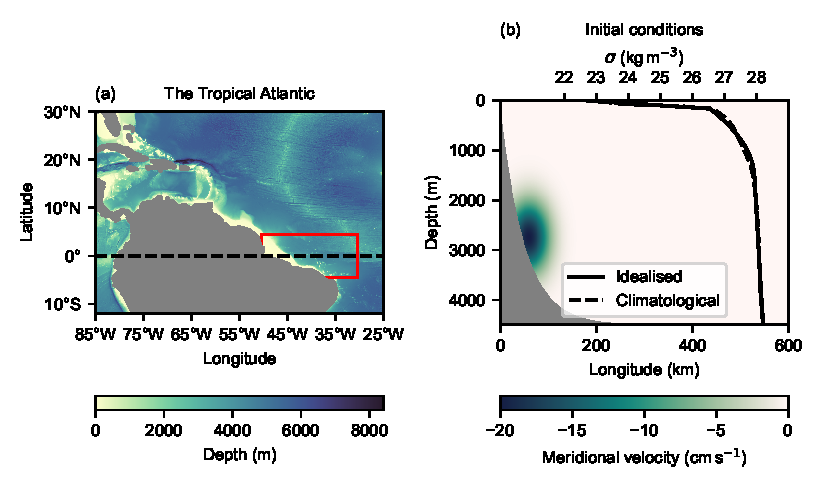
\includegraphics[width=\textwidth]{../figures/Figure1.pdf}
    \caption{(a) Bathymetric map of the western tropical Atlantic. Climatological profiles of neutral density were aggregated from the area enclosed by the red rectangle. Bathymetry data is from the \citet{GEBCO2020} dataset. (b) Meridional velocity (colours) and density (solid line) profiles used as initial and boundary conditions for the model. The velocity profile is based on observations by~\citet{Schott2005}, and the density profile on the climatological mean from~\citet{WOA2018} (dashed line).}
    \label{fig:fig1}
\end{figure}
Simulations of an idealised deep western boundary current crossing the equator are performed using the MITgcm~\citep{Marshall1997}. The domain size is 600 km in the zonal direction, 3,600~km in the meridional and 4,500~m in the vertical. The horizontal grid spacing is 1~km and the vertical grid spacing is 10~m. As with the models of the North Brazil Current, the horizontal resolution is chosen to ensure the model adequately resolves the small-scale vorticity dynamics we are studying and the vertical resolution is chosen to be smaller than the expected size of the overturning cells that symmetric instability generates\footnotemark. The time step is 144~s and the model is integrated for a total of 239~days. The longer integration time is chosen as the slower speeds of the Deep Western Boundary Current mean the model takes longer to spin up. The model domain is sited on a $\beta$-plane, with the equator placed 2,000~km north of the southern boundary. The meridional gradient in the Coriolis parameter is set to $2.3 \times 10^{-11}$ s$^{-1}\,$m$^{-1}$, and the meridional component of the Coriolis parameter is set to $1.5 \times 10^{-4}$ s$^{-1}$.
\footnotetext{A higher horizontal resolution is used here than in the North Brazil Current simulations, as at the time of the integrations being performed I was helping to test the ARCHER2 HPC facility before it came online. I had been instructed to try and push the system in terms of both the number of cores being used and the amount of data being produced. Ramping up the resolution was a simple (if not particularly creative) way of doing this.}

At the surface, a rigid lid boundary condition is employed. The lateral boundary conditions are set to be free-slip and the bottom boundary condition to no-slip. The model has sloping bathymetry as shown in figure~\ref{fig:fig1}b, which also shows the meridional velocity and density profiles used to initialise the model. The zonal velocity is initially set to zero. The density profile is based on a neutral density climatology aggregated from the area enclosed by the red rectangle in figure~\ref{fig:fig1}a. The model is forced by prescribing the meridional velocity, zonal velocity, and density, at the northern and southern domain boundaries. The same fields used to initialise the model are used as boundary conditions. A sponge region is placed at both the northern and southern edges of the domain. The northern sponge is 100 km thick and the southern sponge is 300~km thick. The inverse relaxation timescale varies from $1\times 10^{-5}$~s$^{-1}$ (corresponding to a timescale of around 1.2~days) at the external boundary of the sponge region to 0 at the model-sponge interface. The inverse relaxation timescale has a hyperbolic tangent shape, with a characteristic length scale of 5~km in the northern sponge and 10~km in the southern sponge.

As in chapter~\ref{chap:3}, a linear equation of state is used, with a reference density of 1022.73 kg\,m$^{-3}$ and thermal expansion coefficient of $2 \times 10^{-4}$ K$^{-1}$. The linear equation of state avoids the complexities added by non-linear effects such as thermobaricity and cabbelling~\citep[e.g.][]{Groeskamp2016}. The thermal diffusion coefficient is set to $1 \times 10^{-5}$ m$^{2}$\,s$^{-1}$. A second-order-moment Prather advection scheme with a flux limiter is employed. Salinity is set to be constant and has no impact on the dynamics. Momentum dissipation is provided by a vertical Laplacian viscosity of $4 \times 10^{-4}$ m$^{2}$\,s$^{-1}$ and an adaptive biharmonic Smagorinsky viscosity which acts on horizontal momentum gradients. Potential vorticity is calculated using the C-grid algorithm of~\citet{Morel2019}.

\section{Symmetric instability and staircase formation}
\label{sec:randd}
Figure~\ref{fig:staircase}b shows $\partial_z b$ in the model after 239 days of integration 250 km south of the equator. Immediately apparent are the thin, sharp regions of high stratification (so-called ``mixing barriers'') separating larger regions of well-mixed waters with low and uniform stratification. Moving to 500 km south, we see in figure~\ref{fig:staircase}c that some weaker barriers have dissipated, however, the stronger barriers remain. Figure~\ref{fig:staircase}a shows the squared buoyancy frequency at the equator. At the outer edge of the current's core, we see some weak mixing barriers.

\begin{figure}[t]
    \centering
    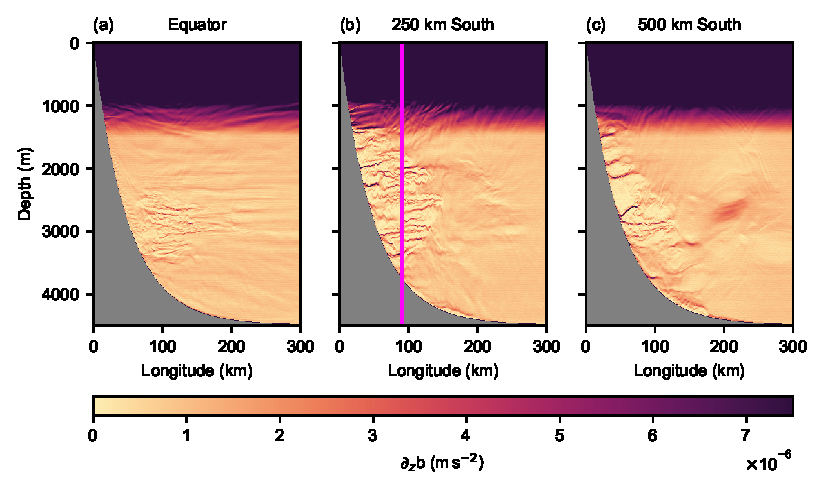
\includegraphics{../figures/Figure2.pdf}
    \caption{Squared buoyancy frequency after 239 days of model integration plotted at (a) the equator,  (b) 250 km south of the equator and (c) 500 km south of the equator. The magenta line indicates the location of the vorticity and density profiles shown in figure~\ref{fig:StaircaseMechanism}.}
    \label{fig:staircase}
\end{figure}

Figure~\ref{fig:StaircaseMechanism}a shows the average of the meridional component of relative vorticity between 234 and 239  days of model integration in a region 250 km south of the equator. This can be thought of as a crude proxy for a zonal overturning stream function --- it measures the local rotation around the meridional axis, i.e. the amount of zonal overturning. As the flow is not invariant in the meridional direction, the ``true'' zonal overturning stream function is ill-defined, so here we will consider the meridional vorticity instead. Examining the meridional vorticity, note that there are a series of counter-rotating stacked overturning cells between around 1,750 m and 3,500 m below the surface. The black contours overlain show $\partial_z b = 2 \times 10^{-6}$~s$^{-2}$ and help identify the locations of the mixing barriers in figure~\ref{fig:staircase}b. We can see that the structure of the buoyancy frequency squared and the meridional vorticity are remarkably similar, with the horizontal edges of the overturning cells (vorticity zeros) approximately coinciding with the locations of the mixing barriers. This can also be seen in figure~\ref{fig:StaircaseMechanism}b. The black line shows neutral density plotted as a function of depth at 250 km south and 90 km west (the location of the magenta lines and points shown in the other figures). The orange line shows the meridional component of relative vorticity at the same point. Both quantities have been averaged over the period spanning 234 to 239 days. The treads of the steps in neutral density correspond to mixing barriers and the risers to well-mixed regions. When comparing neutral density and the meridional vorticity we again see that the mixing barriers tend to coincide with vorticity zeros, whereas the mixing barriers coincide with vorticity extrema. This suggests that the inhomogeneous mixing driven by the overturning cells is what is causing the formation of the staircases.

\begin{figure}[p]
    \centering
    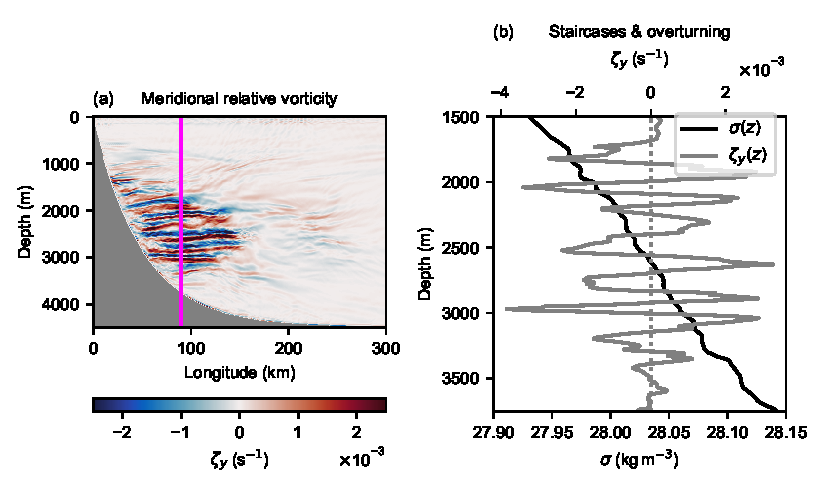
\includegraphics{../figures/Figure3.pdf}
    \caption{(a) The time mean meridional component of relative vorticity between 234 and 239 days of model integration, plotted as a function of longitude and depth, at 250 km south. Overlain is the contour defined by $\partial_z b = 2 \times 10^{-6}$~s$^{-2}$, indicating locations of mixing barriers. (b) Density (black line) and the time mean meridional component of relative vorticity (orange line) plotted as a function of depth at 90 km west and 250 km south (shown on other figures as a magenta line or point). Panels (c) to (e) show snapshots of the stratification over time from the toy model. The contours on panel (c) show the overturning stream function used to drive staircase formation.}
    \label{fig:StaircaseMechanism}
\end{figure}

\subsection{A very simple model of staircase formation}
The differential mixing which produces the mixing barriers is analogous to the process which produces zonal jets on a $\beta$-plane \citep{Manfroi1999}. \citet{Manfroi1999} study a sheared zonal flow on a $\beta$-plane and find that mixing in the presence of a meridional gradient in planetary vorticity leads to the preferential formation of zonal jets. The separation of the jets is set by the strength of the mixing. Here, instead of a meridional gradient in planetary vorticity, there is a vertical gradient in buoyancy and instead of mixing in the horizontal plane we have overturning in the vertical plane. We can reproduce the formation of mixing barriers with a toy model, in which we consider how buoyancy changes over time as a result of vertical diffusion and advection by overturning cells. If we express the overturning motion as a stream-function $\psi$ where $u = - \partial_z \psi$ and $w = \partial_x \psi$ and use a constant harmonic diffusivity, $\kappa$ we can express the evolution of $b$ as
% TODO: Do we need to reparamaterise this now we're using a variable diffusivity?
\begin{equation}
    \frac{\partial b}{\partial t} = \frac{\partial \psi}{\partial z} \frac{\partial b}{\partial x} - \frac{\partial \psi}{\partial x} \frac{\partial b}{\partial z} + \kappa \frac{\partial^2 b}{\partial z^2} \, .
\end{equation}
This is the advection-diffusion equation of a passive tracer in a two-dimensional flow. We choose $\psi = e^{- x^2 / 2\delta_x^2} \sin(m z)$, to represent stacked overturning cells which are localised to a region of width $\delta_x$ in the horizontal. We also set $b(t=0) = N^2 z$, and then solve the equation numerically using the 3rd order Adam's Bashforth scheme on a domain stretching from $-50$~km to $50$~km in the horizontal and spanning $600$~m in the vertical. We set $\delta_x = 25$~km, $m = 2 \pi / 200$ m$^{-1}$, $\kappa = 1 \times 10^{-5}$~m$^2$\,s$^{-1}$ and $N^2 = 1 \times 10^{-6}$~s$^{-2}$. The grid spacing is set to 1 km in the horizontal and 2.5 m in the vertical, and the time step is 240 seconds. In regions where the stratification is unstable, $\kappa$ is increased to $5 \times 10^{-3}$~m$^2$\,s$^{-1}$.

The stratification in this toy model is shown at three different times in figures~\ref{fig:StaircaseMechanism}c to \ref{fig:StaircaseMechanism}e. Alternating high and low stratification regions develop with time. Initially, this is a result of differential mixing; however, at later times the mixing barriers become sharper and start to form filaments due to the extra mixing occurring in regions with unstable stratification.

% TODO: Make the profile point smaller
\begin{figure}[p]
    \centering
    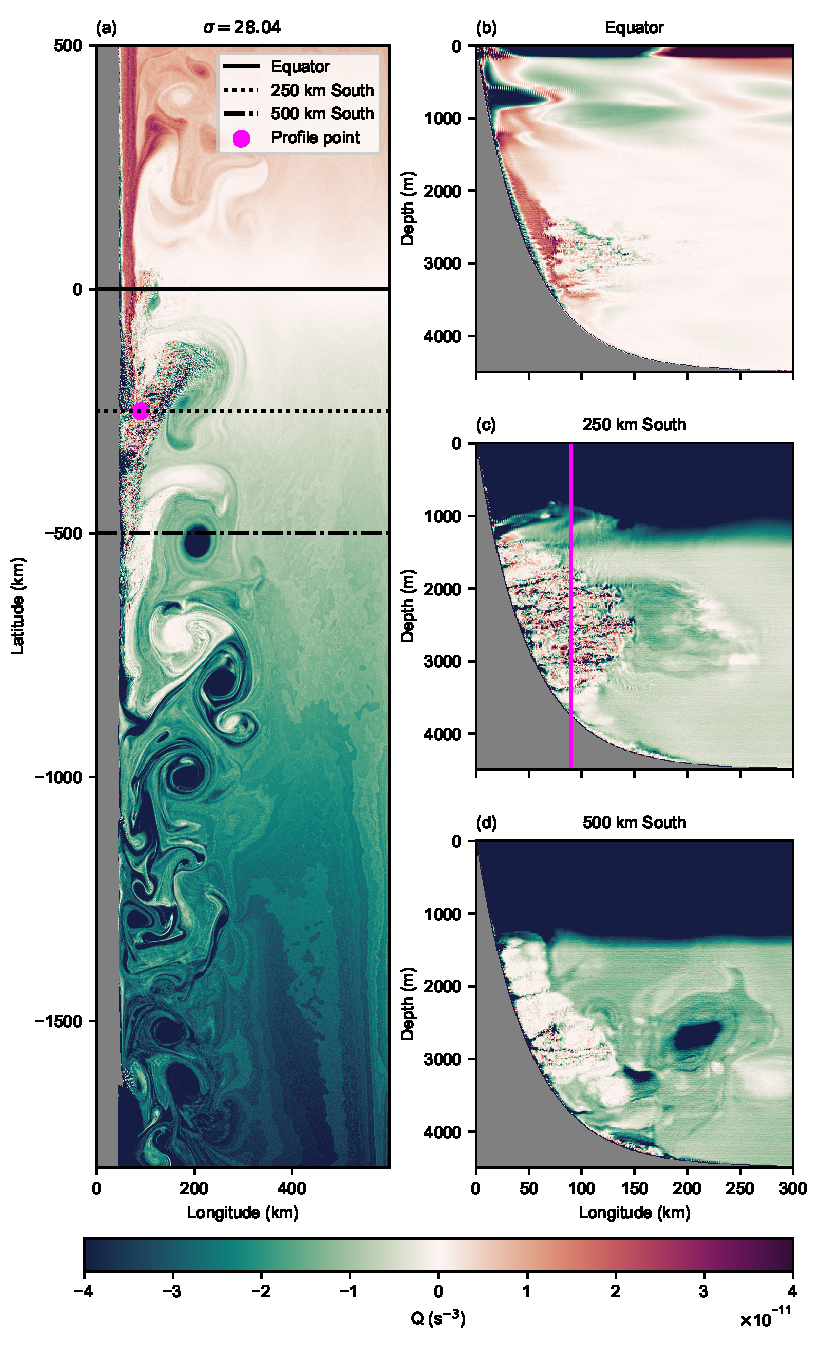
\includegraphics{../figures/Figure4.pdf}
    \caption{Potential vorticity after 239 days of model integration plotted on (a) the $\gamma^n = 28.04$ surface, (b) at the equator, (c) at 250 km south of the equator, and (d) at 500 km south of the equator. Black lines show the latitudes at which sections have been plotted. The magenta line and point indicate the location of the vorticity and density profiles shown in figure~\ref{fig:StaircaseMechanism}.}
    \label{fig:PV}
\end{figure}

\subsection{But what is generating the overturning?}
In chapter~\ref{chap:3}, we saw that western boundary currents can become unstable when crossing the equator as they advect anomalous potential vorticity from one hemisphere into the other. In figure~\ref{fig:PV}a, which shows the potential vorticity on the $\gamma^n$ = 28.04 surface, we can see the advection of positive potential vorticity from the Northern Hemisphere into the Southern Hemisphere, so we may expect to see symmetric instability excited south of the equator. The excitement of the instability is apparent in a region from around 25 km to 600 km south of the equator. Figures~\ref{fig:PV}b to \ref{fig:PV}d show the potential vorticity as a function of depth and longitude at, the equator, 250 km south and 500 km south respectively, after 239 days of model integration. At the equator, we see the advection of waters with anomalous potential vorticity into the Southern Hemisphere. At 250 km south we can see the excitement of symmetric instability, and by 500 km south we can see large pools of neutral potential vorticity suggesting the waters here have experienced symmetric instability, with the excitement of symmetric instability still underway at around 3,000 m. In figure~\ref{fig:PV}b we also see symmetric instability-like patterns in a region of negative potential vorticity. This suggests these waters with negative potential vorticity were undergoing symmetric instability in the Northern Hemisphere before being advected south of the equator. This also explains the presence of the weak staircases at the equator seen in figure~\ref{fig:staircase}a. A similar mechanism was proposed by \citet{DOrgeville2004} in their investigation of deep zonal jets along the equator.

\subsection{Estimating at which latitudes symmetric instability occurs}
\label{sec:relation2nbc}
In the Deep Western Boundary Current, we see the excitement of symmetric instability close to the equator followed by the formation of eddies, unlike in the North Brazil Current where we see the spinning up of large anti-cyclonic eddies followed by the excitement of symmetric instability further away from the equator. This is due to the reduced growth rate of barotropic instability in the deep western boundary current~\citep{Edwards1998II}, meaning that symmetric instability dominates over short time scales. In the North Brazil Current the anti-cyclonic eddies act to reduce the growth rate of symmetric instability further, allowing anomalous potential vorticity to persist whilst the eddies grow~\citep{Buckingham2021}. 

We can be more quantitative about the latitude at which the instability is forming. There is an e-folding timescale, $\tau_e$, associated with symmetric instability which can be converted into an advective meridional length scale, $y$ with the equation $y = V \tau_e$, where V is a typical meridional velocity. From linear stability theory, we know that for a parallel shear flow, like a deep western boundary current the timescale of symmetric instability is given by
\begin{equation}
    \tau_e \sim \Bigg(\beta y \bigg(f + \frac{V}{L_x}\bigg) \Bigg)^{-1/2}
\end{equation}
\citep{Hoskins1974}, and that for the case of an eddy, such as a North Brazil Current ring, the symmetric instability timescale is
\begin{equation}
    \tau_e \sim \Bigg(\beta y \bigg(f + \frac{2 V}{R}\bigg) \Bigg)^{-1/2}
\end{equation}
\citep{Buckingham2021}. We can then convert these expressions to a meridional length scale, giving
\begin{equation}
    y \sim \sqrt[3]{\frac{V L_x}{\beta}} \, ,
    \label{eq:dwbc_y}
\end{equation}
for parallel shear flows, and for an eddy
\begin{equation}
    y \sim \sqrt[3]{\frac{2 V R}{\beta}} \, .
    \label{eq:nbc_y}
\end{equation}
In the case of the eddying flow, we have assumed the meridional velocity is of a similar order of magnitude to the azimuthal velocity. In both expressions, we have assumed $y$ to be small and only considered terms of the lowest order in $y$. We can now evaluate the expressions for the latitude of the onset of symmetric instability. For the Deep Western Boundary Current we choose $V \sim 0.2$ m\,s$^{-1}$, $L_x \sim 30$ km and $\beta \sim 2.3 \times 10^{-11}$~m$^{-1}$\,s$^{-1}$, giving $y \sim 60$ km. For the North Brazil Current rings we choose $V \sim 1$~m\,s$^{-1}$, $R \sim 100$~km and the same value for $\beta$, giving $y \sim 200$ km. These predictions of the latitude of instability are of the same order of magnitude as those we see in the numerical models. In the case of North Brazil Current rings, we see instability at around 400 km north, and in the Deep Western Boundary Current, we see instability from around 25 km south of the equator.

\section{Summary}
\label{sec:conc}
Density staircases are step-like features which become apparent when density is plotted as a function of depth and are common throughout the Earth's oceans. In an idealised model of a deep western boundary current crossing the equator, we see density staircases form. The staircases are generated by overturning cells which are in turn generated by the excitement of symmetric instability as the current crosses the equator. Symmetric instability in cross-equatorial flows is excited due to the advection of anomalous potential vorticity from one hemisphere to another. The stacked overturning cells that generate the staircases are, however, a feature of symmetric instability regardless of what is forcing it, suggesting we may see staircase formation in other symmetrically unstable flows, including when anomalous potential vorticity is induced by frictional torques or diabatic processes. Differences in the latitude of instability between surface intensified western boundary currents and deep western boundary currents can be adequately explained using simple scaling arguments relating the growth rate of symmetric instability to the currents' advective timescales.

It is thought that diapycnal mixing may play an important role in closing the overturning budget of the Atlantic Meridional Overturning Circulation's deep limb. Figures~\ref{fig:staircase} and~\ref{fig:PV} clearly show that vigorous mixing is taking place; however, accurately calculating the amount of mixing that is occurring is tricky. This is due to the importance of secondary Kelvin Helmholtz instabilities in transforming water masses. In order to resolve these processes, we would need a model with around 40 times the resolution used here \citep{Bachman2014}, which is computationally infeasible --- such a model would require at least $10^4$ times more computational resources to run. Simplified two-dimensional models may help in accurately quantifying the induced diapycnal mixing, however.

Density staircases are well documented in the Tropical Atlantic and are often said to form as a result of salt fingering and double diffusive convection (e.g.~\citet{Schmitt1987, Schmitt2005}). In light of this work, we suggest new insights into mixing in the region could be gained by revisiting existing observations and re-examining the origins of observed staircases.

\chapter{Ekman driven symmetric instability in a high latitude western boundary current}
\label{chap:5}
\begin{quote}
    \textit{I was wondering if it would be possible to request a further 60 kCUs?} --- Fraser Goldsworth
\end{quote}

In previous chapters, we have explored the excitement of symmetric instability generated by the change in sign of planetary vorticity at the equator. We will now turn our attention to instabilities generated by changing the sign of potential vorticity. In particular, we will be exploring the role of symmetric instability in deep water formation in the high-latitude Irminger Current. Here, Ekman pumping by down-front winds leads to the steepening of isopycnals and the subsequent generation of negative potential vorticity. OSNAP observations suggest that symmetric instability is excited as a result. In what follows we will use a model to try and answer questions that these observations can not --- namely how important is symmetric instability in the transformation of water masses in the region?

\section{Water mass formation in the Irminger Sea}
The Irminger sea is a something something just off Greenland.
It has recently been revealed by OSNAP observations to be an important region in the formation of dense North Atlantic Deep Waters which make up the lower limb of the AMOC \citet{Lozier2019}. This finding came as a surprise to many, with most models suggesting deep water formation occurs mainly in the adjacent Labrador Sea. As such, there has been a renewed interest in processes that may enhance deep water formation in the Western Sub-polar North Atlantic Ocean.

The Irminger Current is something I will describe in this paragraph when I can get access to the books I need which are paywalled.

The established view is that North Atlantic Deep Waters form as a result of buoyancy forcing --- predominantly air-sea heat fluxes. A recent study by \citet{LeBras2022} challenges this view. They study the effect of strong down-front winds which blow along the Irminger Current and estimate that the Ekman buoyancy flux caused by these winds can be as much as four times stronger than the buoyancy flux resulting from heat loss to the atmosphere (the mechanism by which winds can extract buoyancy from a flow are described in section~\ref{sec:EkmanInst}). The resulting buoyancy loss can lead to the excitement of symmetric instability which is capable of generating mixing and deepening the mixed layer. The winds that drive these events are described now.

The idea of Ekman-induced symmetric instability being an important mechanism in the formation of deep waters in the Sub-polar North Atlantic is not a new one. \citet{Straneo2002} proposed that the wind-driven Ekman buoyancy flux over the Labrador Sea could be around a third of the air-sea buoyancy flux, and that symmetric instability should be taken into account when modelling deep water formation in the region. 

\citet{Spall2016} investigate the effect of down-front winds in an idealised model of the Irminger Current. They integrate both a two-dimensional and three-dimensional hydrostatic model, with $\Delta x = 500$~m and $\Delta z = 1$~m. They force the model with uniform meridional wind stress which is ramped up over seven days, then held constant for the remaining thirteen days of the model integrations. In their models, they observe an Ekman buoyancy flux that sets the potential vorticity to near zero alongside baroclinic instability. These two processes together act to produce water mass transformations, with baroclinic instability (which is only present in the three-dimensional models) greatly enhancing the transformation rates.

The work of \citet{LeBras2022} raises questions about how much water mass transformation is driven by down-front wind events, and whether these highly seasonal events could be a source of AMOC variability. These questions are incredibly difficult to answer with sparse observations, and so we propose the use of idealised models to fill these gaps. Such results could also be used to form the basis of a parameterisation for mixing induced by down-front wind events (although we will not attempt to do this here). The work of \citet{Spall2016} lays the foundations for addressing these questions, however, their study design means it is only able to partially answer them. Their hydrostatic models are too coarse to provide a truly reliable estimate of the mixing induced by symmetric instability. A non-hydrostatic model with a higher resolution is required to resolve the secondary shear instabilities which are known to be important in generating mixing.

Although \citet{Spall2016} set out to model the same barrier wind events investigated by \citet{LeBras2022}, they force their model with a wind stress which is constant following the first seven days of integration. This means both potential vorticity and buoyancy are constantly being extracted from the flow, meaning their models will not reach a steady state, rather; instability will constantly be excited. This means estimates of mixing at later times in their integrations may be either overestimates or underestimates, depending upon whether the pre-conditioning by the wind stress at earlier times enhances or suppresses subsequent mixing. To estimate the effect of a wind event on mixing, we must model it as just that --- an isolated event, with a wind stress which is ramped up and down from some characteristic value over a characteristic period of time.

In section~\ref{sec:Irm2DMeth} we will describe an ensemble of 37 idealised two-dimensional numerical models of the Irminger Current we plan on using to address the above questions. In section~\ref{sec:IrmRef} we will examine in detail one of the ensemble members, before looking at the results from the whole ensemble in section~\ref{sec:IrmEns}. We will summarise the findings in section~\ref{sec:IrmConc}.

\begin{figure} 
    \centering
    \includegraphics{../figures/EnsembleICs.pdf}
    \caption{A camelid}
    \label{fig:EnsembleICs}
\end{figure}

\section{A two-dimensional model of the Irminger current}
\label{sec:Irm2DMeth}
In section~\ref{subsec:2DMethods} we saw a two-dimensional of the North Brazil Current and how it allowed us to probe symmetric instability in a ``clean'' environment, free from noise from baroclinic and barotropic instabilities. In this chapter, we will use similar two-dimensional models to explore symmetric instability in the Irminger current.

We use a non-hydrostatic configuration of the MITgcm~\citep{Marshall1997} to integrate an idealised two-dimensional model of the Irminger current that is symmetric (periodic) in the along-stream direction. The horizontal domain is 150 km wide in the cross-stream direction and 500 m deep. The horizontal and vertical grid spacings are set to 25 m and 1 m respectively. The resolution is set to be high to ensure the Richardson number is sufficiently small that Kelvin-Helmholtz instabilities can be resolved as they are known to be important for obtaining reliable estimates of the amount of diapycnal mixing that is occurring~\citep{Griffiths2003a, Yankovsky2019}. The time step is set to 2 seconds and the model is integrated for a total of 21 days. The model is sited on an $f$-plane with $f$ set to $1.26 \times 10^{-4}$ s$^{-1}$, corresponding to a latitude of $60^\circ$N. 

At the surface, a rigid lid boundary condition is employed, with the lateral and bottom boundaries set to be free-slip. The model has sloping bathymetry, which can be seen in  figure~\ref{fig:EnsembleICs}b. The model is initialised in thermal wind balance, with the velocity and density profiles shown in figure~\ref{fig:EnsembleICs}b. Both of these profiles are based on observations from the OSNAP array \citet{LeBras2022}.

The model is forced using a time-varying along stream wind-stress. The stress is spatially uniform and Gaussian in time, with the form
\begin{equation}
    \tau_y = \tau_0 e^{-\flatfrac{(t - t_{mid})^2}{2\delta_t^2}} \, .
\end{equation}
For the reference integration, $\tau_0 = - 0.5$ N\,m$^{-2}$, $\delta_t = 2.5$ days. For all the models $t_{mid}$ is set to $10.5$ days. The along-front wind stress leads to a steepening of isopycnals and reduction in potential vorticity which may eventually lead to the excitement of symmetric instability, and in extreme cases, pure gravitational instability. To investigate how different wind forcing affect water mass formation and transformation rates, we also integrate an ensemble of simulations using ten different values of $\tau_0$ ranging linearly from $0$ N\,m$^{-2}$ to $-0.75$ N\,m$^{-2}$ and five different values of $\delta_t$ ranging linearly from 0 days to 5 days. This gives a total of 37 different ensemble members.

As in the previous models, a linear equation of state is used, with a reference density of 1027 kg\,m$^{-3}$, a thermal expansion coefficient of $2 \times 10^{-4}$ K$^{-1}$ and no salinity tracer. The thermal diffusion coefficient is set to $1 \times 10^{-5}$ m$^2$\,s$^{-1}$. A second order-moment Prather advection scheme with a flux limiter is employed. Momentum dissipation is provided by an adaptive biharmonic Smagorinsky viscosity of and a vertical Laplacian viscosity of $4 \times 10^{-4}$ m$^2$\,s$^{-1}$.  

\section{The reference integration}
\label{sec:IrmRef}
For the reference integration $\tau_0$ is set to -0.5 N\,m$^{-2}$ and $\delta_t$ to 2.5 days. Figure DECIDEa shows how the wind stress in the model evolves. This wind stress is lower than the typical peak wind stresses seen over the Irminger Current during Wintertime (typically around -2 N\,m$^{-2}$) but is not atypical for less extreme wind events. The period is COMPARE to the period. Wind stresses in the ensemble of models considered here were not increased above $-0.75$ N\,m$^{-2}$ as the model time-step required to ensure stability made the integrations too computationally intensive to perform.

Figure~\ref{fig:EnsStandardPV} shows the potential vorticity in the reference integration after one week, two weeks and three weeks of model runtime. In panel (a) we see how the down-front wind stress has induced an Ekman transport of surface waters towards the shelf, leading to a steepening of isopycnals and generating unstable stratification at the surface. This makes picking apart the contributions to the mixing from gravitational instability and symmetric instability difficult. We counter this difficulty by asserting that gravitational instability \textit{is} symmetric instability and so no separation is necessary. In the surface 25 m or so we can see regions of negative potential vorticity, and just below these areas of low potential vorticity suggesting that mixing is already occurring.

\begin{figure} 
    \centering
    \includegraphics{../figures/run32PV.pdf}
    \caption{A camelid}
    \label{fig:EnsStandardPV}
\end{figure}

A week later, several days after the wind-forcing has peaked, we see this region of low potential vorticity now penetrates deeply, to the bottom of the coastal shelf. Some negative potential vorticity remains, meaning the flow has not yet fully equilibrated.

\begin{figure} 
    \centering
    \includegraphics{../figures/run32Strat.pdf}
    \caption{Stratification in the reference integration.}
    \label{fig:Camelid}
\end{figure}

Finally, after three weeks, we see near zero potential vorticity throughout the upper 75 m of the shelf and shelf-break region. The majority of the negative potential vorticity has now gone, implying the flow has equilibrated following the wind event and reached a new quasi-steady state. Note how much deeper the mixed layer of this new state is, along with the steepness of the isopycnals which implies a sharp increase in the shear of the current.

\begin{figure} 
    \centering
    \includegraphics{../figures/MLD32.pdf}
    \caption{A camelid}
    \label{fig:EnsStandardMLD}
\end{figure}

We will adopt a quantitative definition for the mixed layer depth, as the depth at which the density drops by $0.05$ kg\,m$^{-3}$ relative to the value at the surface. Figure~\ref{fig:EnsStandardMLD}b shows how the mean (solid line) and the maximum (dashed line) mixed layer depth evolves. We see the maximum mixed layer depth increases almost monotonically, reaching the base of the model after around 11 days. This suggests the model could have done with more vertical levels, however; this was not possible due to computational constraints. The mean mixed layer depth also undergoes a net deepening, from around 95 m to 150 m.

The definition of the mixed layer depth employed here is somewhat arbitrary and so in figure~\ref{fig:EnsStandardMLD}c we also show the mean and maximum depths of several isopycnals over time. They are labelled as classes 0 to 3 and correspond to the lower boundaries of the different water mass classes shown in figure~\ref{fig:WaterClass} and defined in table~\ref{tab:Class}. We see that for classes 1 \& 2 there is a large change in the maximum depth, with these isopycnals now reaching the base of the model. The changes in the mean depths are much more modest, however, focussing on classes 1 \& 2 we see there is a shallowing of the isopycnal depth as the wind event gets underway, followed by isopycnal deepening. This is caused by the Ekman transport forcing the upwelling of waters within these classes. The isopycnals then return to slightly deeper depths following the wind event as a result of diapycnal mixing altering the density structure.

\begin{figure} 
    \centering
    \includegraphics[width=\textwidth]{../figures/place-holder.jpeg}
    \caption{Water mass classes at model instantiation}
    \label{fig:WaterClass}
\end{figure}

\begin{table}[]
    \caption{Water mass classes}
    \label{tab:Class}
    \begin{tabular}{lccl}
        \hline
    \multirow{2}{*}{Class} & \multicolumn{2}{c}{$\gamma^n$ (kg\,m$^{-3}$)}  & \multirow{2}{*}{Name}     \\
                           & Lower boundary & Upper boundary &                           \\ \hline \hline
    0                      & 26.92          & None           & shelf waters              \\
    1                      & 26.98          & 26.92          & shelf-break waters        \\
    2                      & 27.05          & 26.98          & upper intermediate waters \\
    3                      & 27.1211        & 27.05          & lower intermediate waters \\
    4                      & None           & 27.1211        & deep waters               \\ \hline
    \end{tabular}
    \end{table}

The effect of mixing on the different water mass classes can be examined through an analysis of the model's volume budget. Figure~\ref{fig:EnsStandardMLD}c which shows the change in volume of each class over time. We see that there is a huge increase in the amount of class 1 shelf-break waters and a decrease in the volumes of class 0, class 2 \& class 3 waters. We can see that the increase in class 2 waters is largely driven by densification of the lightest waters, and to some extent the lightening of dense waters that sit below. The class 4 deep waters remain relatively unmixed. An attempt was made to calculate the instantaneous rate of change of the volumes in each class (the water mass formation rate), however; the signals were too noisy to be able to draw any meaningful conclusions from them\footnotemark. Instead, in figure~\ref{fig:EnsStandardMLD}d we show the formation rate calculated by differentiating the volume anomaly over time. This gives a much smoother signal. We have expressed the units in Sv\,km$^{-1}$ --- this model is a two-dimensional model, so to get an estimate of the transformation rates across the whole length of the Irminger Current, one should multiply the value by $\sim 10^2$ km.
\footnotetext{Apart from, perhaps, that the variance of water mass formation rates is huge!}

NOW HERE WE SHOULD DISCUSS THE FORMATION RATES

Given that \citet{Spall2016} show that baroclinic instability enhances the water mass transformation produced by symmetric instability, it is pertinent to question how reliably the water mass transformation calculations in this model are. The ensemble of models is too computationally expensive to run over a large domain, however; in future work, it would be interesting to examine the water mass transformation rates in a three-dimensional configuration of the reference integration.



\section{An ensemble of models}
\label{sec:IrmEns}
The ensemble of models was forced with wind-stresses ranging in strength from 0~N\,m$^{-2}$ to~0.75 N\,m$^{-2}$ and a duration of between 0 days and 5 days. For each integration, we calculated the change in the mean mixed layer depth\footnotemark~between the start and the end of the model run. We then plot this as a function of wind stress in figure~\ref{fig:DeltaMLD}. The figure shows changes in mixed layer depth behaving very much as expected --- the longer the duration of the wind events, and the higher the maximum wind stress the deeper the mixed layer.
\footnotetext{Defined as before, as the depth at which the density falls below $0.05$ kg\,m$^{-3}$}

\begin{figure} 
    \centering
    \includegraphics{../figures/DeltaMLD.pdf}
    \caption{Change in mixed layer depth between start and end of model integration.}
    \label{fig:DeltaMLD}
\end{figure}

We also calculate the difference between the volume in each water class (as defined above) between the start and end of each model integration --- this is shown in figure~\ref{fig:EnsVolAnom}. We see that in almost all ensemble runs the amount of class 0 and class 2 waters decreases, whilst the amount of class 1 waters increases. This is a result of water mass transformation between these classes. During the five-day wind events, at higher wind stresses the amount of class 2 waters decreases more than during the shorter wind events, whereas the amount of class 3 waters increases. This is due to the surface buoyancy forcing being strong enough to produce mixing at depth.

\begin{figure} 
    \centering
    \includegraphics{../figures/EnsembleVolAnom.pdf}
    \caption{Volume anomaly in the ensemble. Move legend to axs1 position. Change $\Delta V$ to $\Delta Volume$ possibly with the curly V notation.}
    \label{fig:EnsVolAnom}
\end{figure}

We can differentiate the volume anomaly time series for each class and ensemble member, to give formation rates. Figure~\ref{fig:EnsPkFormation} shows the mean, maximum and minimum formation rates for each ensemble member, in units of Sv\,km$^{-1}$. We would like to be able to plot the water mass transformation as a function of density, however; the presence of unstable stratification makes performing the calculations in density space difficult (if not impossible). NOW DESCRIBE WHAT WE SEE.

\begin{figure} 
    \centering
    \includegraphics{../figures/EnsembelPeakFormation.pdf}
    \caption{Maybe this would be better with envelopes for the standard deviation of the tendency over time.}
    \label{fig:EnsPkFormation}
\end{figure}


\section{Implications \& conclusions}
\label{sec:IrmConc}
\chapter{Conclusions}
\begin{quote}
    \textit{You live and learn. At any rate, you live.} --- Douglas Adams
\end{quote}
This thesis set out to investigate the role of symmetric instability in different western boundary current systems, which act as important pathways for waters participating in the basin-scale AMOC. In particular, we focussed on the North Brazil Current and the Deep Western Boundary Current as they cross the equator, and the East Greenland Current during winter and spring-time barrier wind events.

In chapter~\ref{chap:1}, we examined the importance of the AMOC and saw how mixing in its many constituent currents is of fundamental importance to its large-scale dynamics. We learnt how symmetric instability can be an efficient way to generate sub-mesoscale motions capable of mixing buoyancy, momentum, potential vorticity and other tracers of interest in currents with potential vorticity opposite in sign to that of the planetary vorticity. We outlined how this mixing may go some way toward solving the ``cross-equatorial flow problem''. The crux of this problem is that in order for large-scale interhemispheric water exchanges to occur, there must exist a process capable of changing the sign of the potential vorticity of the waters crossing the equator \citet{Killworth1991}. The conservation of potential vorticity, however, places limits on the kinds of processes which may modify potential vorticity and requires the mechanism to move velocity and buoyancy gradients towards dissipative scales. The AMOC's climatic importance is partly derived from its role in facilitating the interhemispheric transport of waters and so solving this problem is of fundamental importance. Away from the equator, we saw how observations of symmetric instability in the East Greenland Current show that the instability is capable of producing significant deepening of the mixed layer there, but that these observations leave questions about the amount of diapycnal mixing the instability can generate unanswered.

This leads us to chapter~\ref{chap:2}, where we took an in-depth look at symmetric instability and its properties. We explored two different ways of exciting it --- by either changing the sign of the planetary vorticity or changing the sign of the potential vorticity of a fluid parcel. The first mechanism for generating symmetric instability is unique to currents which cross the equator. A water parcel stable to symmetric instability in one Hemisphere will not be stable to symmetric instability in the opposing Hemisphere. This instability can be generated outside the surface and bottom boundary layers where potential vorticity forcing occurs, making symmetric instability generated in this way distinct from instability generated by buoyancy or momentum forcing.

We then examined how Ekman buoyancy forcing by down-front wind events can generate anomalous potential vorticity and hence symmetric instability (although alternate methods of generating anomalous potential vorticity exist). Geostrophically balanced currents have outcropping isopycnals. When the wind blows along these currents, the surface waters experience Ekman transport perpendicular to the wind, which can act to steepen the isopycnals. If the winds are sufficiently strong this can lead to a change in sign of the potential vorticity. This mechanism has been observed to be at play in the East Greenland Current.

In the following sections we explored where the symmetric instability criterion comes from, examined the orientation of the overturning cells generated by the instability, and looked at gravitational and inertial instabilities as limiting cases of symmetric instability --- symmetric instability can be interpreted as inertial instability along isopycnals or gravitational instability along vortex tubes. This led us to an examination of the energetics of the instability, which in turn informed a discussion of the ``classical'' and ``energetic'' definitions of symmetric instability. In this thesis, we employed the classical definition of symmetric instability, in which gravitational, inertial and slantwise convective instabilities are different ``flavours'' of symmetric instability.

These previous results were derived by considering a symmetric Eady type problem, that of a parallel shear flow \citep{Eady1949, Ooyama1966, Hoskins1974, Stone1966}. We then looked at the axisymmetric problem, which can be thought of as modelling the behaviour of eddies. We saw how rotation modifies the instability criterion, with the cores of anticyclonic eddies being stabilised by the additional centrifugal forces \citep{Buckingham2021}. Having reviewed the established theory of symmetric instability, we broke new ground, applying linear stability analyses to both the North Brazil Current and its rings and the Deep Western Boundary Current as they cross the equator. We used these results to make predictions about the timescales at play and the structures we may see when these currents cross the equator. Although some strong assumptions were made in the application of theory to these real-world currents, the theory's predictions were invaluable in identifying symmetric instability in the more complex numerical models subsequently presented. We see great potential in the use of simple numerical models, like those developed here, in diagnosing symmetric instability in observations and more-realistic General Circulation Model outputs. Using linear theory we were also able to challenge the assumption that the complete Coriolis force would modify the properties of symmetric instability in flows such as the North Brazil Current as they cross the equator. Building on the work of \citet{Zeitlin2018a} we identified a new measure of the importance of the complete Coriolis force on a symmetrically unstable flow, which takes into account its direction. We also defined a class of forces that leave the structure and growth rates of symmetric instabilities unchanged, leading to a more comprehensive understanding of the kinds of forces that can be neglected when studying symmetric instabilities.

In chapter~\ref{chap:3}, we examined symmetric instability in the North Brazil Current, investigating the instability's role in ridding the current of anomalous potential vorticity originating in Southern Hemisphere waters and in generating diapycnal mixing. Through the use of high-resolution modelling, we were able to demonstrate the effect of symmetric instability in setting the absolute vorticity of the flow to zero. Most General Circulation Models neutralise the anomalous potential vorticity of Southern Hemisphere Waters as they cross the equator through lateral dissipation provided by an eddy viscosity \citep{Edwards1998I}. That the effect of the instability is to set the absolute vorticity of the flow to zero suggests that, to first order, such a viscosity may parameterise the process adequately within coarse resolution models. A caveat to this is that our model is likely underestimating water mass transformation rates which affect the density structure. This is due to the resolution being too coarse to resolve secondary Kelvin-Helmholtz instabilities which are known to be important in the generation of water mass transformations by symmetric instability \citep[e.g.][]{Yankovsky2019, Griffiths2003a, Taylor2009}. Despite this limitation, our models still show symmetric instability can produce a large amount of mixing, with up to 2~Sv worth of transformation between surface and intermediate waters and between 2~Sv and 4~Sv of transformation between intermediate and deep waters. Due to the nature of symmetric instability in cross-equatorial western boundary currents, this transformation is occurring continuously, meaning symmetric instability may be important in transforming surface waters into deep waters in the Tropical Atlantic. The water mass transformation rates, as opposed to the formation rates, will give a more reliable assessment of the importance of symmetric instability in generating mixing, however, these calculations are more computationally expensive to perform. It would also be interesting to investigate these rates in more realistic models of the Tropical Atlantic such as the GIGATL \citep{Gula2021a} and MITgcm LLC4320 \citep{Forget2015} models\footnotemark.
\footnotetext{We did attempt to do this in 2020, however, were beset by problems accessing a small subset of the large quantities of data these models produce. Significant progress has been made since then though --- see for example the Poseidon project \citep{Haine2021} and proposals from the Pangeo project \citep{Uchida2022} which aim to address these issues.}

In chapter~\ref{chap:4} we examined the excitement of symmetric instability in the Deep Western Boundary Current as it crossed the equator. We showed that despite the growth rate of symmetric instability in the current being very small (due to the smallness of both the planetary vorticity and the relative vorticity of the current) symmetric instability is still excited and sets the potential vorticity of the flow to zero. If this prediction of the presence of symmetric instability in the Deep Western Boundary Current is borne out by observations, it will be one of the first examples of symmetric instability occurring away from either the surface or bottom boundary layers of the ocean. This work also predicted the latitudes at which we expect the instability to be most active, which may aid in searching for observational evidence of its excitement. We also demonstrated that symmetric instability (or any other overturning instability in a stratified flow) can lead to the generation of density staircases. A clear next step in searching for observational evidence of symmetric instability in the Deep Western Boundary Current would be to analyse existing CTD casts in the region which may show step-like features with a length scale of between approximately 10~m to 250~m. Furthermore, the linear theory of chapter~\ref{chap:2} demonstrated the link between the vertical step height of the staircase (set by the height of the overturning cells) and the rate at which secondary instabilities dissipate momentum --- as parameterised by a vertical viscosity. Applying the linear theory to observed currents as an inverse-type model would enable an estimation of the viscosity which is best used for parameterising the secondary shear instabilities which equilibrate unstable flows. Such a viscosity may serve as a crude first-order parameterisation of Kelvin-Helmholtz instability in general circulation models of sufficient resolution to permit symmetric instability. The finding in chapter~\ref{chap:4} that symmetric instability is occurring much closer to the equator (around 25~km away) in the Deep Western Boundary Current than in the North Brazil Current (around 400~km away) is a great vindication of the power of linear theory. Simple scaling arguments were able to predict these numbers before any modelling had taken place.

Finally, in chapter~\ref{chap:5} we investigated the role of Ekman-driven symmetric instability in the East Greenland Current. We showed that strong down-front wind events have a significant impact on the depth of the upper convectively mixed layer and the deeper low potential vorticity layer through the excitement of symmetric instability, and the subsequent diapycnal mixing it generates. Baroclinic instability was not present in the idealised models used to study the process, so it remains to be seen how significant the enhancement of the mixing by baroclinic instability is \citep{Spall2016}. That the winds can generate up to 2 Sv of mixing (when integrated over the length of the East Greenland Current) suggests that the instability may explain some short timescale overturning variability seen in AMOC observations at the OSNAP East array. Despite the significant amounts of instantaneous diapycnal mixing generated by down-front wind events in our model, it is clear that the wind events themselves are not frequent enough for the amount of diapycnal mixing generated to account for more than a few tenths of a Sverdrup of deep water formation when integrated over the length of the current and a 12-month period. However, this is not to say that the process is insignificant. The deepening and restratification of the mixed layer during these wind events may be important in pre-conditioning surface waters, ready for other processes to transform them into North Atlantic Deep Waters --- this should be investigated further. In particular, the role of baroclinic instability in producing further mixing should be investigated, although other mixed layer instabilities could also be important.

Significantly, chapter~\ref{chap:5} suggests that a simple mixed layer parameterisation of gravitational instability, such as KPP, may adequately represent the mixing produced by Ekman-induced symmetric instability in the East Greenland Current.
This is due to the high latitude meaning the zero potential vorticity state is very close to a zero stratificaiton state. The effectiveness of such a parameterisation should be evaluated and compared to the results we present here, as should the effectiveness of parametrisations specifically targeted at representing the effects of symmetric instability.
The KPP parameterisation is already implemented in many climate and general circulation models, meaning minimal work would be required to ensure we are adequately representing the re-stratifying effects of down-front winds.

This thesis has examined the role of symmetric instability in three very different currents --- the surface intensified North Brazil Current, the much slower Deep Western Boundary Current as it crosses the equator, and the highly baroclinic East Greenland Current. Symmetric instabilities are often seen as sitting on a spectrum, with gravitational instability at one end and inertial instability at the other. We have explored both extremes of the spectrum in this work and, I hope, demonstrated how a classical definition of symmetric instability aids in understanding this class of overturning instabilities. We have seen how symmetric instability plays a role in the mixing of buoyancy, momentum and potential vorticity in each of these currents. These three currents, however, are only a small subset of those which combine to form the AMOC. The role of submesoscale instability in many other currents which contribute to this global scale circulation is yet to be examined. Our understanding of the interior cross-equatorial pathways in the Tropical Atlantic remains incomplete --- in part due to the difficulty in making observations resulting from the breakdown of geostrophy \citep[see e.g.][]{Vianna2003}. Our understanding of deep water formation sites and processes in the Sub-polar North Atlantic is increasing year on year, with unprecedented observations from the ONSAP array revealing the complexity of the circulations in the Sub-polar North Atlantic. In short, theory and models still have a way to go to provide a complete description of the AMOC. It is only by utilising observations when developing theory (as in chapter~\ref{chap:5}) or by utilising theory to inform observations (as we hope to with the staircases seen in chapter~\ref{chap:4}) that we will be able to answer the most pressing questions in the field of AMOC science.

It is imperative that we both understand, and are able to adequately model the ocean's response to anthropogenic climate change. Small-scale processes are key to determining the amount of heat and carbon the ocean will take up \citep{DeLavergne2022}, while the large-scale circulation will determine how these tracers are redistributed across the globe \citep{Buckley2015}. The impacts of the AMOC on the climate system can only truly be appreciated when we think about the largest and smallest scales together.


\pagestyle{fancy}
\fancypagestyle{plain}{%
  \renewcommand{\headrulewidth}{0pt}
  \fancyhf{}
  \fancyfoot[C]{\usefont{T1}{PTSans-TLF}{m}{n}{\thepage}}
}
\renewcommand{\headrulewidth}{0pt}
\fancyhf{}
\fancyfoot[C]{\usefont{T1}{PTSans-TLF}{m}{n}{\thepage}}

\chapter*{Software \& data}
\addcontentsline{toc}{chapter}{Software \& data}
This work was made possible by several open-source pieces of software. These include MITgcm~\citep{MITgcm2022}, xarray~\citep{Hoyer2017}, dask~\citep{DaskDevelopmentTeam2016, Rocklin2015}, xmitgcm~\citep{Abernathey2021}, zarr~\citep{Miles2022}, numpy~\citep{Harris2020}, scipy~\citep{Virtanen2020}, matplotlib~\citep{Hunter2007} and cartopy~\citep{Elson2022}.

The codes used to produce all figures and run all model integrations are available from \citet{dwbcV1p1, irmingerV1p0, nbcV1p0, siV1p0}. Selected model outputs have been archived at \citet{ThesisData}.

\chapter*{List of symbols}
\addcontentsline{toc}{chapter}{List of symbols}

\section*{Greek letters}
\begin{longtable}{cp{\textwidth}}
    $\alpha_T$ & Thermal expansion coefficient \\
    $\beta$ & Meridional gradient of planetary vorticity \\
    $\Gamma$ & The non-traditionality parameter \\
    $\gamma^n$ & Neutral density \\
    $\delta_b$ & Bickley jet width \\
    $\Delta \psi$ & Net volume flux out of a region \\
    $\zeta$ & Absolute vorticity \\
    $\theta$ & Latitude \\
    $\kappa$ & Buoyancy diffusion coefficient \\
    $\lambda$ & Vertical wavelength \\
    $\lambda^*$ & Vertical wavelength which maximises $\sigma$ for a given $A_r$ \\
    $\mathbf{\xi}$ & Relative vorticity, $\curl{\mathbf{u}}$ \\
    $\xi$, $\xi_y$ & Vertical and meridional components of relative vorticity \\
    $\Pi$ & Geopotential pressure \\
    $\rho, \rho_0$ & Density and reference density \\
    $\sigma$ & A growth rate \\
    $\tau$ & $\tan\Phi$ \\
    $\tau_e$ & e-folding timescale \\
    $\tau_y$ & Meridional wind stress \\
    $\Phi$ & Angle of disturbance to the horizontal \\
    $\Phi_{iso}$ & Isopycnal slope \\
    $\chi$ & Angle of coastline to a meridian \\
    $\psi$ & An overturning stream function \\
    $\hat{\psi}$ & The horizontal component of a separable overturning stream function \\
    $\omega$ & An oscillatory frequency, or growth rate if imaginary \\
\end{longtable}

\section*{Latin letters}
\begin{longtable}{cp{\textwidth}}
    $A_r$ & Vertical viscosity \\
    $b$ & Buoyancy \\
    $d$ & An advective length scale \\
    $D_t$ & Material (advective) derivative \\
    $\partial_{t'}$ & $\partial_t - A_r \partial^2_{zz}$ \\
    $E_k$ & Kinetic energy \\
    $\mathbf{f}$ & Planetary vorticity vector \\
    $f$ & Coriolis parameter, the vertical component of planetary vorticity \\
    $f_0$ & Planetary vorticity on an f-plane \\
    $f'$ & Modified Coriolis parameter, $f + 2 \flatfrac{V_\phi}{r}$ \\
    $F_{NT}$ & The meridional or non-traditional component of planetary vorticity. \\
    $\mathcal{F}_x, \mathcal{F}_z$ & Zonal and meridional components of a force \\
    $\mathscr{F}$ & Water mass formation rate \\
    $g$ & Gravitational acceleration \\
    $G$ & Diapycnal volume flux \\
    $H$ & A vertical length scale \\
    $k$ & A horizontal wavenumber or wavenumber magnitude \\
    $L$ & A horizontal length scale \\
    $m$ & A vertical wavenumber \\
    $N^2, M^2$ & Vertical and horizontal derivatives of buoyancy \\
    $P$ & Geopotential pressure \\
    $Q$ & Ertel potential vorticity \\
    $r, \phi, z$ & Cylindrical polar coordinates \\
    Sv & Sverdrup --- unit of $1 \times 10^{6}$~m$^3$\,s$^{-1}$ \\
    $t$ & time \\
    $T$, $T_0$ & Temperature, reference temperature \\
    $u, v, w$ & Cartesian components of velocity \\
    $v_r, v_\phi, w$ & Cylindrical polar components of velocity \\
    $\mathcal{V}$ & Volume enclosed by two isopycnals \\
    $x, y, z$ & Cartesian coordinates \\
\end{longtable}
    

%now enable appendix numbering format and include any appendices
%\appendix
%\include{appendix1}
%\include{appendix2}

%next line adds the Bibliography to the contents page
\addcontentsline{toc}{chapter}{Bibliography}
%uncomment next line to change bibliography name to references
\renewcommand{\bibname}{References}
\bibliography{library}        %use a bibtex bibliography file refs.bib
\bibliographystyle{agsmdoi}  %use the plain bibliography style

\end{document}